\documentclass[11pt,]{article}
\usepackage{lmodern}
\usepackage{amssymb,amsmath}
\usepackage{ifxetex,ifluatex}
\usepackage{fixltx2e} % provides \textsubscript
\ifnum 0\ifxetex 1\fi\ifluatex 1\fi=0 % if pdftex
  \usepackage[T1]{fontenc}
  \usepackage[utf8]{inputenc}
\else % if luatex or xelatex
  \ifxetex
    \usepackage{mathspec}
    \usepackage{xltxtra,xunicode}
  \else
    \usepackage{fontspec}
  \fi
  \defaultfontfeatures{Mapping=tex-text,Scale=MatchLowercase}
  \newcommand{\euro}{€}
\fi
% use upquote if available, for straight quotes in verbatim environments
\IfFileExists{upquote.sty}{\usepackage{upquote}}{}
% use microtype if available
\IfFileExists{microtype.sty}{%
\usepackage{microtype}
\UseMicrotypeSet[protrusion]{basicmath} % disable protrusion for tt fonts
}{}
\usepackage[margin=1in]{geometry}
\usepackage{color}
\usepackage{fancyvrb}
\newcommand{\VerbBar}{|}
\newcommand{\VERB}{\Verb[commandchars=\\\{\}]}
\DefineVerbatimEnvironment{Highlighting}{Verbatim}{commandchars=\\\{\}}
% Add ',fontsize=\small' for more characters per line
\usepackage{framed}
\definecolor{shadecolor}{RGB}{248,248,248}
\newenvironment{Shaded}{\begin{snugshade}}{\end{snugshade}}
\newcommand{\KeywordTok}[1]{\textcolor[rgb]{0.13,0.29,0.53}{\textbf{{#1}}}}
\newcommand{\DataTypeTok}[1]{\textcolor[rgb]{0.13,0.29,0.53}{{#1}}}
\newcommand{\DecValTok}[1]{\textcolor[rgb]{0.00,0.00,0.81}{{#1}}}
\newcommand{\BaseNTok}[1]{\textcolor[rgb]{0.00,0.00,0.81}{{#1}}}
\newcommand{\FloatTok}[1]{\textcolor[rgb]{0.00,0.00,0.81}{{#1}}}
\newcommand{\CharTok}[1]{\textcolor[rgb]{0.31,0.60,0.02}{{#1}}}
\newcommand{\StringTok}[1]{\textcolor[rgb]{0.31,0.60,0.02}{{#1}}}
\newcommand{\CommentTok}[1]{\textcolor[rgb]{0.56,0.35,0.01}{\textit{{#1}}}}
\newcommand{\OtherTok}[1]{\textcolor[rgb]{0.56,0.35,0.01}{{#1}}}
\newcommand{\AlertTok}[1]{\textcolor[rgb]{0.94,0.16,0.16}{{#1}}}
\newcommand{\FunctionTok}[1]{\textcolor[rgb]{0.00,0.00,0.00}{{#1}}}
\newcommand{\RegionMarkerTok}[1]{{#1}}
\newcommand{\ErrorTok}[1]{\textbf{{#1}}}
\newcommand{\NormalTok}[1]{{#1}}
\usepackage{longtable,booktabs}
\usepackage{graphicx}
\makeatletter
\def\maxwidth{\ifdim\Gin@nat@width>\linewidth\linewidth\else\Gin@nat@width\fi}
\def\maxheight{\ifdim\Gin@nat@height>\textheight\textheight\else\Gin@nat@height\fi}
\makeatother
% Scale images if necessary, so that they will not overflow the page
% margins by default, and it is still possible to overwrite the defaults
% using explicit options in \includegraphics[width, height, ...]{}
\setkeys{Gin}{width=\maxwidth,height=\maxheight,keepaspectratio}
\ifxetex
  \usepackage[setpagesize=false, % page size defined by xetex
              unicode=false, % unicode breaks when used with xetex
              xetex]{hyperref}
\else
  \usepackage[unicode=true]{hyperref}
\fi
\hypersetup{breaklinks=true,
            bookmarks=true,
            pdfauthor={},
            pdftitle={rapr: Representative and Adequate Prioritisations in R},
            colorlinks=true,
            citecolor=blue,
            urlcolor=blue,
            linkcolor=magenta,
            pdfborder={0 0 0}}
\urlstyle{same}  % don't use monospace font for urls
\setlength{\parindent}{0pt}
\setlength{\parskip}{6pt plus 2pt minus 1pt}
\setlength{\emergencystretch}{3em}  % prevent overfull lines
\setcounter{secnumdepth}{0}

%%% Use protect on footnotes to avoid problems with footnotes in titles
\let\rmarkdownfootnote\footnote%
\def\footnote{\protect\rmarkdownfootnote}

%%% Change title format to be more compact
\usepackage{titling}

% Create subtitle command for use in maketitle
\newcommand{\subtitle}[1]{
  \posttitle{
    \begin{center}\large#1\end{center}
    }
}

\setlength{\droptitle}{-2em}
  \title{rapr: Representative and Adequate Prioritisations in R}
  \pretitle{\vspace{\droptitle}\centering\huge}
  \posttitle{\par}
  \author{Jeffrey O. Hanson$^1$, Jonathan R. Rhodes$^2$, Hugh P. Possingham$^1$,
Richard A. Fuller$^1$\\$^1$School of Biological Sciences, The University
of Queensland, Brisbane, QLD, Australia\\$^2$School of Geography,
Planning and Environmental Management, The University of Queensland,
Brisbane, QLD, Australia\\Correspondance should be addressed to
\href{mailto:jeffrey.hanson@uqconnect.edu.au}{jeffrey.hanson@uqconnect.edu.au}}
  \preauthor{\centering\large\emph}
  \postauthor{\par}
  \predate{\centering\large\emph}
  \postdate{\par}
  \date{26 February 2016}

% load packages
\usepackage{amsmath,amsfonts,float,makecell,titletoc,tocloft,titlesec,natbib,pdfpages,lineno}
\usepackage[T1]{fontenc}
\usepackage{lmodern}
\usepackage[utf8]{inputenc}
\usepackage[doublespacing]{setspace}

% format captions
\usepackage[labelfont={small,bf}, labelsep=space, font={small}]{caption}

% format headings
\titleformat{\subsection}
{\normalfont\Large\bfseries}{\thesubsection}{1em}{}
\titleformat{\subsubsection}
{\normalfont\large\bfseries}{\thesubsubsection}{1em}{}
\titleformat{\paragraph}
{\normalfont\normalsize\bfseries}{\theparagraph}{1em}{}
\titleformat{\subparagraph}
{\normalfont\normalsize\itshape}{\thesubparagraph}{1em}{}

\titlespacing\paragraph{0pt}{12pt plus 4pt minus 2pt}{+0pt plus 2pt minus 2pt}
\titlespacing{\subparagraph}{0pt}{6pt plus 4pt minus 2pt}{+0pt plus 2pt minus 2pt}

% format toc
\renewcommand\cftsubsecfont{\normalfont\normalsize\bfseries}
% \renewcommand\cftsubsubsecfont{\normalfont\normalsize\bfseries}
% \renewcommand\cftparafont{\normalfont\normalsize\bfseries}
% \renewcommand\cftsubparafont{\normalfont\normalsize\itshape}

% make figures static
\let\origfigure\figure
\let\endorigfigure\endfigure
\renewenvironment{figure}[1][2] {
	\expandafter\origfigure\expandafter[H]
} {
	\endorigfigure
}


\begin{document}

\maketitle

\begin{abstract}
A central aim in conservation is to maximise the long-term persistence
of biodiversity. To fulfil this aim, reserve networks are used to
safeguard biodiversity patterns (eg. species, populations) and processes
(eg. evolutionary processes that underpin genetic variation). Reserve
selection is often formulated as an optimisation problem to identify
cost-effective prioritisations. However, most existing decision support
tools are based on formulations that are well suited for preserving
biodiversity patterns, but not biodiversity processes. To fill this gap
in the conservation planning toolbox, we developed the \texttt{rapr} R
package. This R package provides functions to solve reserve selection
problems using two novel formulations. Here, we explore the
functionality of this R package using simulated species and a
conservation planning exercise in Queensland, Australia as a case-study.
We demonstrate how explicitly considering biodiversity processes can
alter a prioritisation. In most cases, we found that only a few
additional plannning units are required to sufficiently preserve of
biodiversity processes.
\end{abstract}

Short running title: Representative and adequate prioritizations
\newline
Word count: XXXXX \newline
Number of references: XXXX \newline
Number of figures, table and text boxes: 4 \newline
\newpage

\newpage
\setcounter{tocdepth}{5} \hypersetup{linkcolor=black} \tableofcontents
\newpage

\subsection{Introduction}\label{introduction}

The overarching aim of conservation is to maximise the long-term
persistence of biodiversity (McNeely 1994; Margules and Pressey 2000).
To achieve this, conservation actions must preserve biodiversity
patterns (eg. species, populations) and the processes that sustain them.
One of the major tangible achievements of modern conservation has been
the act of setting aside areas for preservation (Sanderson \emph{et al.}
2015). Reserve networks buffer species from threatening processes
{[}Margules and Pressey (2000); eg. urbanisation{]} and set the stage
for direct management interventions (eg. captive breeding and
reintroduction programs; Kleiman 1989). However, the resources available
for conservation action are limited, and so reserve networks must be
sited in places that satisfy conservation objectives for minimum cost
(Margules and Pressey 2000). To achieve this, reserve selection is often
formulated as an optimisation problem and then solved to identify
cost-effective candidate reserve systems (prioritisations; Margules and
Pressey 2000).

To fulfil the overarching aims of conservation, reserve networks must
preserve both ecological and evolutionary processes (Margules and
Pressey 2000; Crandall \emph{et al.} 2000). Ecological processes, such
as predator-prey interactions, pollination, and decomposition, are
required for biodiversity to persist over short time-scales. Typically,
they operate over small geographic domains--with exceptions such as
migration and refugial habitats--and can be preserved using suitably
large planning units (Ciarleglio \emph{et al.} 2009) that each contain a
discrete unit of habitat (Klein \emph{et al.} 2009). On the other hand,
evolutionary processes are required for biodiversity to persist over
long time-scales, and they typically operate over large geographic
domains. Adaptive evolutionary processes can be preserved by securing
populations with different adaptations and/or along selection pressure
gradients (eg. environmental gradients; Moritz 2002; Crandall \emph{et
al.} 2000; Rouget \emph{et al.} 2003; Cowling \emph{et al.} 2003).
Neutral evolutionary processes can be preserved by securing populations
with different evolutionary histories and/or with limited gene flow
(Moritz 2002; Carvalho \emph{et al.} 2011; Ponce-Reyes \emph{et al.}
2014). Due to advances in technology in recent decades, a wealth of data
on biodiversity processes has become freely available to conservation
planners. Yet this data is only rarely used to guide conservation
planning exercises (Hendry \emph{et al.} 2010). Existing decision
support tools focus primarily on preserving biodiversity patterns or
occasionally processes--but not both.

Many tools have been developed to assist conservation planners in
preserving biodiversity patterns (eg. \texttt{C-Plan}, Pressey \emph{et
al.} 2009;\texttt{ ConsNet}, Ciarleglio \emph{et al.}
2009;\texttt{ Marxan}, Ball \emph{et al.} 2009;\texttt{ Zonation},
Moilanen 2007). They use targets (eg. \texttt{Marxan}) or weights (eg.
\texttt{Zonation}) to identify prioritisations that contain an adequate
amount of individuals or habitat for a set of species (features). To
accommodate information on biodiversity processes, conservation planners
can split features into sub-features as a pre-processing step (eg.
Carvalho \emph{et al.} 2011). However, this approach is limited because
data on biodiversity processes is often continuous and hyper-dimensional
(eg. bioclimatic data; Hijmans \emph{et al.} 2005), and therefore they
often cannot be reduced to a few categories without significant
information loss (Faith and Walker 1996). Additionally, these problem
formulations cannot accommodate variation within sub-features, and nor
can they account for relationships between sub-features (Faith and
Walker 1996).

Very few tools have been developed with a specific focus on biodiversity
processes. The \texttt{DIVERSITY} decision support tool (Faith 2003)
uses continuous data to site reserves in places that secure a
representative sample of variation across a study area (eg.
environmental variation). Originally, this tool was developed to
identify prioritizations that secure a comprehensive set of habitats
without using any species-level data. As a consequence, the
effectiveness of this tool has been highly contested ({{Araújo}}
\emph{et al.} 2001, 2003; Faith 2011). Additionally, this tool tended to
deliver excessively fragmented prioritisations (cf. \texttt{Marxan}).
However, unlike tools that primarily focus on biodiversity patterns,
this tool can only accommodate data on the distribution of a single
feature.

Today, one of the key issues preventing decision makers from explicitly
considering both biodiversity patterns and processes in the reserve
selection process is the lack of a decision support tool that can
accommodate data on both in a multi-species context. To fill this void,
we present the \texttt{rapr R} package. This \texttt{R} package provides
decision makers with the tools to identify prioritisations that preserve
biodiversity patterns and processes. These prioritisations are generated
by solving novel formulations of the reserve selection problem that use
adequacy- and representation-based targets. We also provide a tutorial
showcasing the functionality of this \texttt{R} package using simulated
species and a case-study conservation planning scenario in Queensland,
Australia.

\subsection{Problem formulations}\label{problem-formulations}

The \texttt{rapr R} package uses two novel formulations of the reserve
selection problem to identify cost-effective prioritisations. These
formulations share many constraints and variables. For brevity, the
variables used by both formulations will be defined. Biodiversity
features are defined as the entity(s) that the prioritisation is
required to preserve (eg. species, populations). Spatial attributes are
defined as the intra-feature variation that the prioritisation is
required to sample. These attributes are related to the biodiversity
processes that the prioritisation needs to represent (eg. environmental
variation).

Each attribute is conceptualised as a space and planning units are
thought to occupy points inside each space. This space is termed an
attribute space. For example, a decision maker may require a
prioritisation that preserves populations along climatic gradients. To
achieve this, the decision maker might use an ``climatic'' attribute
space with dimensions relating to mean annual temperature ($^{\circ}$C)
and precipitation (mm). Any given combination of temperature and
precipitation may be conceived as a point in this environmental space.
By associating planning units with climatic data, they can be mapped
from geographic space to this environmental attribute space.

Demand points are points that exist in an attribute space. They are
designated by the decision maker to indicate regions of the attribute
space that should be preserved in the prioritisation. The amount of
variation in the attribute space that a prioritisation secures is a
function of the distance between each demand point and each planning
unit in the attribute space. The shorter the distances between the
demand points and the planning units; the better the prioritisation is
at representing the variation in the spatial attribute. To convert these
amounts to a proportion--a meaningful unit for a decision maker--the
distances between the selected planing units and the demand points are
scaled by the distances between the demand points to the centroid of the
demand points. In any attribute space there may exist points that are
impossible (eg. mean annual rainfall -5 mm), do not occur in the study
area (eg. mean annual temperature 30$^{\circ}$C in Antarctica), or are
undesirable (eg. conditions known to be outside the physiological
tolerance of a species). By placing demand points in desirable regions
of an attribute space, the decision maker can ensure that
prioritisations secure desirable values of a spatial attribute.

To illustrate these concepts, we will briefly describe a conservation
planning scenario example involving attribute spaces and demand points.
A decision maker may wish to develop a prioritisation for a single
species. This species has four populations in the study area. These
populations are in the process of divergent evolution, with different
populations inhabiting different environmental conditions and accruing
different adaptations. However, the decision maker can only afford to
preserve three of the populations. The decision maker needs to select a
set of populations that will secure the most of intra-specific
variation. To describe this intra-specific variation--given that no
genetic data was available--the decision maker obtained data on the
environmental conditions (rainfall (ml) and temperature ($^{\circ}$C))
where each population was found. The decision maker then used this
environmental data to construct a two-dimensional environmental
attribute space. Next, the decision maker generated demand points as
equi-distant points between the range of values where the populations
were found ($\pm$ 20\% to avoid edge effects; Faith and Walker 1996). By
comparing the distribution of the demand points to the distribution of
the populations in the attribute space, the decision maker can identify
a suitable prioritisation (Figure 1). We can see that if the decision
maker preserves both populations $A$ and $C$, they will effectively
``double-up'' on the same environmental characteristics, and in turn
their waste resources. Instead, a more representative sample of the
intra-specific variation could be preserved by securing populations $A$,
$B$, and $D$. This example demonstrates how the inclusion of
biodiversity processes can guide the reserve selection process.

\begin{figure}[htbp]
\centering
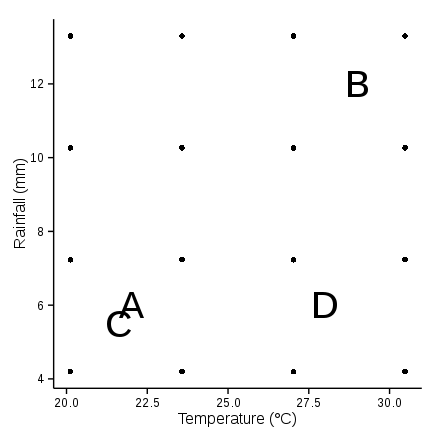
\includegraphics{rapr_files/figure-latex/unnamed-chunk-1-1.pdf}
\caption{Example of an attribute space. This environmental attribute
space has dimensions relating to annual temperature ($^{\circ}$C)and
rainfall (ml) values. Letters denote the environmental conditions
associated with the geographic locations where four hypothetical
populations are found. Points represent demand points. In this space,
populations closer to each other are considered more similar to each
other.}
\end{figure}

The problem formulations used to guide reserve selection in the
\texttt{rapr R} package are based on a combination of the
\texttt{Marxan} reserve selection problem and uncapacitated facility
location problems (all mathematical terms defined hereafter are
described in Table S1 for convenience). For convenience, the cardinality
of sets will be denoted using the same symbol used to denote the
variable. Define $F$ to be the set of features (indexed by $f$). Let $J$
be a set of planning units (indexed by $j$). Also, let $A_j$ denote the
area, and $C_j$ denote the cost of preserving planning unit $j \in J$.
To assess the extent to which each feature is secured in a given
prioritisation, let $q_{fj}$ denote the probability of feature $f$
occupying planning unit $j$. The level of fragmentation associated with
a prioritisation is parametrised as the net exposed boundary length. Let
the shared boundary length between each planning unit $j \in J$ and
$k \in J$ be $b_{jk}$. In any real-world problem, some planning units
will have edges that are not associated with any neighbouring planning
units (eg. edges along coastlines), these cases will be denoted using
$b_{jj}$ for $j \in J$.

Let $S$ denote a set of attribute spaces (indexed by $s$). Each
$j \in J$ is associated with spatially explicit data that represent
coordinates for each attribute space $s \in S$. Let $I_{fsi}$ denote a
set of demand points (indexed by $i$) for each feature $f \in F$ and
each attribute space $s \in S$. Let $\lambda_{fsi}$ denote the weighting
for each demand point $i \in I$, $f \in F$ and $s \in S$. Let $d_{fsij}$
denote the distance between each demand point $i \in I$ and each
planning unit $j \in J$ for each feature $f \in F$ and attribute space
$s \in S$. Let $\hat{d}_{fsi}$ denote the distance between each demand
point $i \in I$ and the centroid of the demand points. Demand points
with greater weight $\lambda_{fsi}$ are more important, and the optimal
solution will be likely to select planning units close to highly
weighted demand points. As a consequence, the decision maker will need
to choose an appropriate weighting for each demand point. The decision
maker will also need to choose an appropriate distance metric for each
attribute space. For example, Euclidean, Mahalanobis (Mahalanobis 1936),
Bray-Curtis, or other distance metrics may be appropriate given the
nature of the attribute space (Faith \emph{et al.} 1987).

Targets are used to ensure that prioritisations adequately preserve each
species. Amount-based targets are used to ensure that the total amount
of habitat preserved is sufficient. Let $\hat{T}_f$ denote the expected
amount of area that needs to be preserved for each feature $f \in F$.
Space-based targets are ensure that a sufficient proportion of the
intra-specific variation is secured. Let $\bar{T}_{fs}$ denote the
space-based targets for feature $f \in F$ and attribute space $a \in A$.
For convenience, these both types of targets are expressed as
proportions in the \texttt{R} package.

The \texttt{R} package provides two formulations for reserve selection.
They are based on the unreliable (Fernández and Landete 2015) and
reliable uncapacitated facility location (Cui \emph{et al.} 2010)
problems. The key difference between them is that the reliable
formulation explicitly considers the probability that the planning units
are occupied when calculating the proportion of variation that a given
solution secures, whereas the unreliable formulation does not.

\subsubsection{Unreliable formulation}\label{unreliable-formulation}

In the unreliable formulation, the control variables are the $BLM$,
$\hat{t}_{s}$, and $\bar{t}_{sa}$ variables, and the decision variables
are the $X_j$ and $Y_{fsi}$ variables.

\begin{align*}
X_j
    &= \begin{cases}
        1, & \text{if planning unit $j$ is selected for conservation action} \tag{1a} \\
        0, & \text{otherwise} \\
    \end{cases} \\
%
\hat{T}_s &= \text{amount target for feature $f$} \tag{1b}\\
%
\bar{T}_{sa} &= \text{representation target for feature $f$ in attribute space $a$} \tag{1c}\\
%
BLM &= \text{boundary length modifier: penalises overly fragmented solutions} \tag{1d}\\
Y_{fsi} &= \begin{cases}
        1, & \text{if planning unit $i$ is assigned to planning unit $j$ for feature $f$ in space $s$} \tag{1e} \\
        0, & \text{otherwise} \\
    \end{cases} \\
\end{align*}

The unreliable formulation (URAP) is a defined as a multi-objective
optimisation problem.

\begin{align*}
& \text{(URAP)} & \text{Min } & \sum_{j=0}^{J-1} C_j + BLM \times \sum_{j=0}^{J-1} \sum_{k=j}^{J-1} X_j \left( 1-X_k \right) b_{jk} + & & \tag{2a} \\
& & & BLM \times \sum_{j=0}^{J-1} x_j b_{jj} & & & \\
%
& & \text{s.t. } & \sum_{j=0}^{J-1} A_j q_{jf} \geq \bar{T}_{f} & \forall & 0 \leq f \leq F-1 \tag{2b}\\
%
& & & 1 - \frac{\sum_{i=0}^{I-1} \sum_{j=0}^{J-1} \left( \lambda_{fsi} d_{fsij} Y_{fsij} \right)^2}{\sum_{i=0}^{I-1} \left( \lambda_{fsi} \hat{d}_{fsi} \right)^2 } \geq \hat{T}_{fs}  & \forall & 0 \leq f \leq F-1, \tag{2c}\\
& & & & & 0 \leq s \leq S-1\\
%
& & & \sum_{j=0}^{J-1} Y_{fsij} = 1 & \forall & 0 \leq f \leq F-1, \tag{2d}\\
& & & & & 0 \leq s \leq S-1, \\
& & & & & 0 \leq i \leq I-1\\
%
& & & Y_{fsij} \leq X_j & \forall & 0 \leq f \leq F-1, \tag{2e}\\
& & & & & 0 \leq s \leq S-1, \\
& & & & & 0 \leq i \leq I-1,\\
& & & & & 0 \leq j \leq J-1\\
%
& & & X_j, Y_{fsij} \in {0,1} & \forall & 0 \leq f \leq F-1, \tag{2f}\\
& & & & & 0 \leq s \leq S-1,\\
& & & & & 0 \leq i \leq I-1\\
%
\end{align*}

The objective function (2a) determines the utility of a given
prioritisation: a combination of the total cost of a prioritisation and
how fragmented it is. Constraints (2b--2c) ensure that all the
amount-based and space-based targets are met. Constraints (2d) ensure
that only one planning unit is assigned to each demand point.
Constraints (2e) ensure that demand points are only assigned to selected
planning units. Constraints (2f) ensure that the $X$ and $Y$ variables
are binary.

\subsubsection{Reliable formulation}\label{reliable-formulation}

The reliable formulation explicitly considers the probability that the
planning units are inhabited. As a consequence, it may deliver
prioritisations that will sufficiently represent an attribute space even
if the features do not inhabit several of the planning units when the
prioritisation is implemented. This behaviour is achieved by siting
back-up planning units near selected planning units with low occupancy
probabilities in the attribute space(s). To ensure that prioritisations
are robust against multiple planning units being uninhabited, the
problem assigns planning units at multiple backup levels.

Backup levels levels are defined as $r$-levels (similar to failure
levels in Snyder and Daskin 2005). The first backup $r$-level is used to
calculate the level of representation when all of the selected planning
units are occupied by all $f \in F$. For this scenario, the closest
selected planning unit to each demand point $i$ for attribute space $s$
is assigned at $r$-level$=0$. This scenario essentially represents
$Y_{fsij}$ in the unreliable formulation. The second backup $r$-level is
used to assess the level of representation when the closest planning
unit to each demand point $i$ is unoccupied. For this scenario, the
second closest planning units are assigned at $r$-level$=1$. The third
backup $r$-level is used to assess representation when the first two
closest planning units are unoccupied. The third closest planning units
are assigned at $r$-level$=2$. Continuing on, in this manner, the
selected planning units in a prioritisation are assigned to each demand
point $i \in I$, attribute space $s \in S$, and each feature $f \in F$
at an $r$-level.

A final backup $r$-level when $r=R$ is used to assess the level of
representation when the features $f \in F$ do not occupy any selected
planning units in a prioritisation. Each demand point $i \in I$ for each
$s \in S$ and $f \in F$ is assigned to an ``imaginary'' planning unit
$j=J$ at $r=R$. The distance variables associated with this imaginary
planning unit $d_{fsiJ}$ denote the loss of biological value associated
with failing to secure a representative sample of feature $f$ in
attribute space $s$. However, the $d$ variables are in distance units
which are meaningless units in this context. Thus these variables are
calculated using a failure multiplier ($M$) and the maximum distance
between the planning units and the demand points for $f \in F$,
$s \in S$ (3).

\begin{align*}
& d_{fsiJ} = M \times \max\limits_{0 \leq i \leq I-1, 0 \leq j \leq J-1} d_{fsij} & \forall & 0 \leq f \leq F-1, \tag{3} \\
& & & 0 \leq s \leq S-1\\
\end{align*}

Moderately-sized conservation planning problems often include several
thousand planning units. It is currently not be feasible to solve this
problem when considering all possible failure scenarios. As a
consequence, the $R$ variable can be any $1 \leq R \leq J-1$. For
instance, when $R=3$ only 2 backup levels are considered in addition to
the final backup level. Cui et al. (2010) found that $R=5$ yields
similar solutions to $R=J$ when $J >> 5$. However, depending on the
number of features, demand points, attribute spaces, and planning units,
decision makers will likely be limited to $R=1$ to obtain
prioritisations in a feasible amount of time.

In the reliable formulation, the control variables are the $BLM$,
$\hat{t}_{s}$, $\bar{t}_{sa}$, $R$, and $M$ variables. The decision
variables are the $X_j$, $Y_{fsijr}$, $P_{fsijr}$ variables.

\begin{align*}
& \text{(1a--1d)} \\
R &= \text{number of failure levels} \tag{4a} \\
%
M &= \text{failure multiplier} \tag{4b}\\
%
P_{fsijr} &= \parbox{25em}{probability that demand point $i$ is assigned to planning unit $j$ at back-up level $r$ for feature $f$ and space $s$} \tag{4c}\\
\end{align*}

The reliable formulation (RRAP) is a multi-objective optimisation
problem.

\begin{align*}
& \text{(RRAP)} & \text{Min } & \text{(2a)}\\
%
& & \text{s.t. } & \text{(2b)}\\
%
& & & 1 - \frac{\sum_{i=0}^{I-1} \sum_{j=0}^{J-1} \left( \lambda_{fsi} d_{fsij} P_{fsijr} Y_{fsij} \right)^2}{\sum_{i=0}^{I-1} \left( \lambda_{fsi} \hat{d}_{fsi} \right)^2 } \geq \hat{T}_{fs}  & \forall & 0 \leq f \leq F-1, \tag{5a}\\
& & & & & 0 \leq s \leq S-1\\
%
& & & \sum_{j=0}^{J-1} Y_{fsijr} = 1 & \forall & 0 \leq f \leq F-1, \tag{5b}\\
& & & & & 0 \leq s \leq S-1,\\
& & & & & 0 \leq i \leq I-1,\\
& & & & & 0 \leq r \leq R\\
%
& & & \sum_{r=0}^{R} Y_{fsijr} = 1 & \forall & 0 \leq f \leq F-1, \tag{5c}\\
& & & & & 0 \leq s \leq S-1,\\
& & & & & 0 \leq i \leq I-1,\\
& & & & & 0 \leq j \leq J\\
%
& & & \sum_{r=0}^{R-1} Y_{fsijr} \leq X_j & \forall & 0 \leq f \leq F-1, \tag{5d}\\
& & & & & 0 \leq s \leq S-1,\\
& & & & & 0 \leq i \leq I-1,\\
& & & & & 0 \leq j \leq J-1\\
%
& & & Y_{fsiJR} = 1 & \forall & 0 \leq f \leq F-1, \tag{5e}\\
& & & & & 0 \leq s \leq S-1,\\
& & & & & 0 \leq i \leq I-1\\
%
& & & P_{fsij0} = q_{fj} & \forall & 0 \leq f \leq F-1, \tag{5f}\\
& & & & & 0 \leq s \leq S-1,\\
& & & & & 0 \leq i \leq I-1,\\
& & & & & 0 \leq j \leq J\\
%
& & & P_{fsijr} = \left(1 - \right) \sum_{k=0}^{J-1} \frac{1 - q_k}{q_k} P_{f,s,i,k,r-1} Y_{f,s,i,k,r-1}  & \forall & 0 \leq f \leq F-1, \tag{5g}\\
& & & & & 0 \leq s \leq S-1,\\
& & & & & 0 \leq i \leq I-1,\\
& & & & & 0 \leq j \leq J,\\
& & & & & 1 \leq r \leq R\\
%
& & & X_j, Y_{fsijr} \in {0,1} & \forall & 0 \leq f \leq F-1, \tag{5h}\\
& & & & & 0 \leq s \leq S-1,\\
& & & & & 0 \leq i \leq I-1,\\
& & & & & 0 \leq j \leq J,\\
& & & & & 0 \leq r \leq R\\
\end{align*}

The objective function for the reliable formulation is the same as for
the unreliable formation (2a). Similar to the unreliable formulation,
constraints (2b) and (5a) ensure that the amount-based and space-based
targets are met. Constraint (5b--5c) ensure that each planning unit is
only assigned to one backup $r$-level for $i \in I$. Constraints (5d)
ensure that only selected planning units are assigned to demand points
$i \in I$. Constraints (5e) ensure that the imaginary planning unit is
always assigned to the highest backup $r$-level. Constraints (5f--5g)
determine the probability that planning unit $j$ will be used to sample
demand point $i \in I$ for $s \in S$ and $f \in F$ (Cui \emph{et al.}
2010). Constraints (5h) ensure that the $X$ and $Y$ variables are
binary.

\subsubsection{Optimisation}\label{optimisation}

The unreliable and reliable formulations are non-linear. However, the
non-linear components can be linearised using existing techniques.
First, the expression $X_j X_k$ in (2a) can be linearised using methods
described by Beyer et al. (2015). Second, the expression
$P_{fsijr} Y_{jsijr}$ in (5a) can be linearised using techniques
described by Sherali and Alameddine (1992) as implemented in Cui et al.
(2010). Linearised versions of the problems can be solved using
commercial exact algorithm solvers.

The \texttt{rapr} R package provides functions to express conservation
planning data as an optimisation problems using linearised versions of
the unreliable and reliable formulations. These optimisation problems
can then be solved to generate prioritisations using the commercial
\texttt{Gurobi} software suite (\url{http://www.gurobi.com}). Note that
academics can obtain a
\href{http://user.gurobi.com/download/licenses/free-academic}{license at
no cost from the Gurobi website}. After installing the \texttt{Gurobi}
software suite, users will need to install the \texttt{Gurobi R}
package. This \texttt{R} package can be installed on
\href{http://www.gurobi.com/documentation/6.5/quickstart_windows/r_installing_the_r_package.html}{Windows},
\href{http://www.gurobi.com/documentation/6.5/quickstart_mac/r_installing_the_r_package.html}{Mac
OSX}, and
\href{http://www.gurobi.com/documentation/6.5/quickstart_linux/r_installing_the_r_package.html}{Linux}
operating systems.

\subsection{Package overview}\label{package-overview}

To load the \texttt{rapr} R package and learn more about the package,
type the following code into R.

\begin{Shaded}
\begin{Highlighting}[]
\CommentTok{# load rapr R package}
\KeywordTok{library}\NormalTok{(rapr)}

\CommentTok{# show package overview}
\NormalTok{?rapr}
\end{Highlighting}
\end{Shaded}

The \texttt{rapr} R package uses a range of S4 classes to store
conservation planning data, parameters, and prioritisations (Table 1).

Table 1: Main classes in the \texttt{rapr} R package

\begin{longtable}[c]{@{}cll@{}}
\toprule\addlinespace
Class Name & Description & Slots
\\\addlinespace
\midrule\endhead
ManualOpts &
\makecell[l]{place-holder class for manually specified solutions} &
\makecell[l]{NumberSolutions}
\\\addlinespace
GurobiOpts &
\makecell[l]{parameters for solving optimisation\\problems using Gurobi}
& \makecell[l]{Threads, MIPGap,\\Presolve, TimeLimit,\\NumberSolutions}
\\\addlinespace
RapUnreliableOpts &
\makecell[l]{parameters for the unreliable problem formulation} &
\makecell[l]{BLM}
\\\addlinespace
RapReliableOpts &
\makecell[l]{parameters for the reliable problem formulation} &
\makecell[l]{failure.multiplier,\\max.r.level}
\\\addlinespace
SimplePoints &
\makecell[l]{stores coordinates in an n-dimensional space} &
\makecell[l]{coords}
\\\addlinespace
DemandPoints &
\makecell[l]{demand points coordinates and weights\\for a speciesin an attribute space}
& \makecell[l]{points, weights}
\\\addlinespace
AttributeSpace &
\makecell[l]{planning unit coordinates and demand\\points data for an attribute space}
& \makecell[l]{pu, demand.points,\\distance.metric}
\\\addlinespace
RapData & \makecell[l]{planning unit, species, and attribute space data}
&
\makecell[l]{pu, species, targets,\\pu.species.probabilities,\\attribute.spaces,\\boundary, polygons,\\.cache}
\\\addlinespace
RapUnsolved &
\makecell[l]{data and parameters needed to generate\\prioritisationsusing RAP}
& \makecell[l]{opts, data}
\\\addlinespace
RapResults & \makecell[l]{prioritisations and summary statistics} &
\makecell[l]{summary, selections,\\amount.held, space.held,\\logging.file, .cache}
\\\addlinespace
RapSolved &
\makecell[l]{data, parameters, and prioritisations using them} &
\makecell[l]{opts, data, results}
\\\addlinespace
\bottomrule
\end{longtable}

\subsection{Package tutorial}\label{package-tutorial}

This tutorial is designed to provide users with an understanding of how
to use the \texttt{rapr R} package to generate and compare solutions.
This tutorial uses several additional packages, so first we will run the
following code to load them.

\begin{Shaded}
\begin{Highlighting}[]
\CommentTok{# load packages for tutorial}
\KeywordTok{library}\NormalTok{(plyr)}
\KeywordTok{library}\NormalTok{(dplyr)}
\KeywordTok{library}\NormalTok{(ggplot2)}
\KeywordTok{library}\NormalTok{(RandomFields)}

\CommentTok{# set seed for reproducibility}
\KeywordTok{set.seed}\NormalTok{(}\DecValTok{500}\NormalTok{)}
\end{Highlighting}
\end{Shaded}

\subsubsection{Simple simulated species}\label{simple-simulated-species}

\paragraph{Data}\label{data}

To investigate the behaviour of the problem, we will generate
prioritisations for three simulated species. We will use the unreliable
formulation of the problem to understand the basics, and later move onto
the reliable formulation. The first species (termed `uniform') will
represent a hyper-generalist. This species will inhabit all areas with
equal probability. The second species (termed `normal') will represent a
species with a single range core. The third species (termed `bimodal')
will represent a species with two distinct ecotypes, each with their own
range core. To reduce computational time for this example, we will use a
10 $\times$ 10 grid of square planning units.

\begin{Shaded}
\begin{Highlighting}[]
\CommentTok{# make planning units}
\NormalTok{sim_pus <-}\StringTok{ }\KeywordTok{sim.pus}\NormalTok{(100L)}

\CommentTok{# simulate species distributions}
\NormalTok{sim_spp <-}\StringTok{ }\KeywordTok{lapply}\NormalTok{(}
    \KeywordTok{c}\NormalTok{(}\StringTok{'uniform'}\NormalTok{, }\StringTok{'normal'}\NormalTok{, }\StringTok{'bimodal'}\NormalTok{),}
    \NormalTok{sim.species,}
  \DataTypeTok{n=}\DecValTok{1}\NormalTok{,}
  \DataTypeTok{x=}\NormalTok{sim_pus,}
  \DataTypeTok{res=}\DecValTok{1}
\NormalTok{)}
\end{Highlighting}
\end{Shaded}

Let's see what these species' distributions look like.

\begin{Shaded}
\begin{Highlighting}[]
\CommentTok{# plot species}
\KeywordTok{plot}\NormalTok{(}
    \KeywordTok{stack}\NormalTok{(sim_spp),}
    \DataTypeTok{main=}\KeywordTok{c}\NormalTok{(}\StringTok{'Uniform species'}\NormalTok{,}\StringTok{'Normal species'}\NormalTok{,}\StringTok{'Bimodal species'}\NormalTok{),}
    \DataTypeTok{addfun=}\NormalTok{function()\{}\KeywordTok{lines}\NormalTok{(sim_pus)\},}
    \DataTypeTok{nc=}\DecValTok{3}
\NormalTok{)}
\end{Highlighting}
\end{Shaded}

\begin{figure}[htbp]
\centering
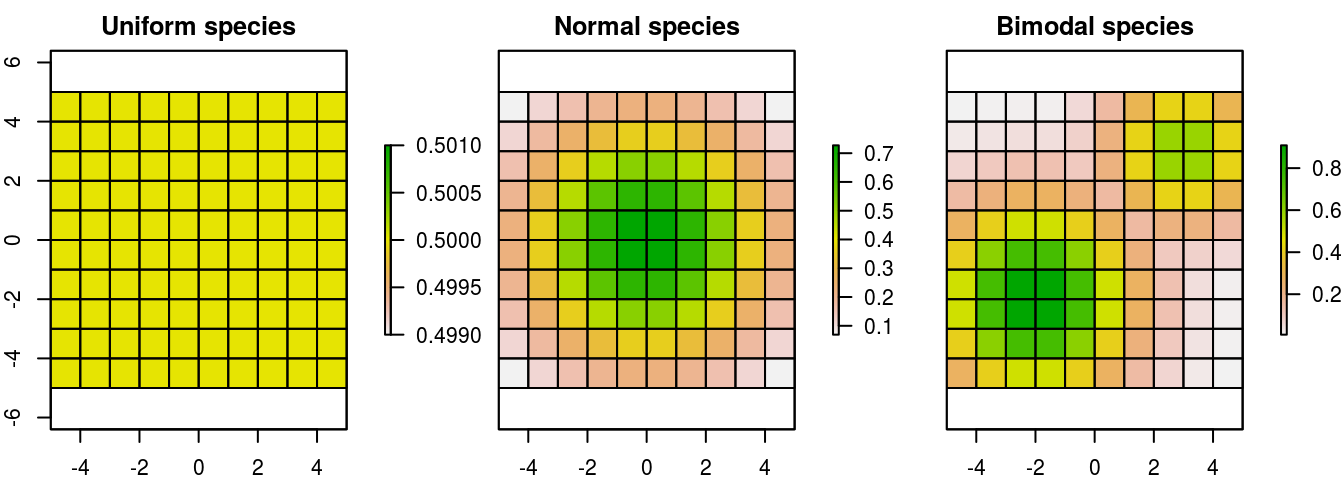
\includegraphics{rapr_files/figure-latex/unnamed-chunk-5-1.pdf}
\caption{Distribution of three simulated species. Each square represents
a planning unit. The colour of each square denotes the probability that
individuals from each species occupy it.}
\end{figure}

Next, we will generate a set of demand points. To understand the effects
of probabilities and weights on the demand points, we will generate the
demand points in geographic space. These demand points will be the
centroids of the planning units. Additionally, we will use the same set
of demand points for each species and only vary the weights of the
demand points between species. \textbf{Note that we are only using the
same distribution of demand points for different species for teaching
purposes. It is strongly recommended to use different demand points for
different species in real-world conservation planning exercises.} See
the case-study section of this tutorial for examples on how to generate
suitable demand points.

\begin{Shaded}
\begin{Highlighting}[]
\CommentTok{# generate coordinates for pus/demand points}
\NormalTok{pu_coords <-}\StringTok{ }\NormalTok{rgeos::}\KeywordTok{gCentroid}\NormalTok{(sim_pus, }\DataTypeTok{byid=}\OtherTok{TRUE}\NormalTok{)}

\CommentTok{# calculate weights}
\NormalTok{sim_dps <-}\StringTok{ }\KeywordTok{lapply}\NormalTok{(}
    \NormalTok{sim_spp,}
    \NormalTok{function(x) \{}
        \KeywordTok{return}\NormalTok{(}\KeywordTok{extract}\NormalTok{(x, pu_coords))}
    \NormalTok{\}}
\NormalTok{)}

\CommentTok{# create demand point objects}
\NormalTok{sim_dps <-}\StringTok{ }\KeywordTok{lapply}\NormalTok{(}
    \NormalTok{sim_dps,}
    \NormalTok{function(x) \{}
        \KeywordTok{return}\NormalTok{(}
            \KeywordTok{DemandPoints}\NormalTok{(}
                \KeywordTok{SimplePoints}\NormalTok{(pu_coords@coords),}
                \KeywordTok{c}\NormalTok{(x)}
            \NormalTok{)}
        \NormalTok{)}
    \NormalTok{\}}
\NormalTok{)}
\end{Highlighting}
\end{Shaded}

Now, we will construct a \texttt{RapUnsolved} object to store our input
data and parameters. This contains all the information to generate
prioritisations.

\begin{Shaded}
\begin{Highlighting}[]
\NormalTok{## create RapUnreliableOpts object}
\CommentTok{# this stores parameters for the unreliable formulation problem (eg. BLM)}
\NormalTok{sim_ro <-}\StringTok{ }\KeywordTok{RapUnreliableOpts}\NormalTok{()}

\NormalTok{## create RapData object}
\CommentTok{# create data.frame with species info}
\NormalTok{species <-}\StringTok{ }\KeywordTok{data.frame}\NormalTok{(}
  \DataTypeTok{name=}\KeywordTok{c}\NormalTok{(}\StringTok{'uniform'}\NormalTok{, }\StringTok{'normal'}\NormalTok{, }\StringTok{'bimodal'}\NormalTok{)}
\NormalTok{)}

\NormalTok{## create data.frame with species and space targets}
\CommentTok{# amount targets at 20% (denoted with target=0)}
\CommentTok{# space targets at 20% (denoted with target=1)}
\NormalTok{targets <-}\StringTok{ }\KeywordTok{expand.grid}\NormalTok{(}
  \DataTypeTok{species=}\DecValTok{1}\NormalTok{:}\DecValTok{3}\NormalTok{,}
  \DataTypeTok{target=}\DecValTok{0}\NormalTok{:}\DecValTok{1}\NormalTok{,}
  \DataTypeTok{proportion=}\FloatTok{0.2}
\NormalTok{)}

\CommentTok{# calculate probability of each species in each pu}
\NormalTok{pu_probabilities <-}\StringTok{ }\KeywordTok{calcSpeciesAverageInPus}\NormalTok{(sim_pus, }\KeywordTok{stack}\NormalTok{(sim_spp))}

\NormalTok{## create AttributeSpace object}
\CommentTok{# this stores the coordinates of the planning units in an attribute space}
\CommentTok{# and the coordinates and weights of demand points in the space}
\NormalTok{attr_space <-}\StringTok{ }\KeywordTok{AttributeSpace}\NormalTok{(}
  \KeywordTok{SimplePoints}\NormalTok{(pu_coords@coords),}
  \NormalTok{sim_dps}
\NormalTok{)}

\CommentTok{# generate boundary data information}
\NormalTok{boundary <-}\StringTok{ }\KeywordTok{calcBoundaryData}\NormalTok{(sim_pus)}

\NormalTok{## create RapData object}
\CommentTok{# this stores all the input data for the prioritisation}
\NormalTok{sim_rd <-}\StringTok{ }\KeywordTok{RapData}\NormalTok{(}
  \NormalTok{sim_pus@data,}
  \NormalTok{species,}
  \NormalTok{targets,}
  \NormalTok{pu_probabilities,}
  \KeywordTok{list}\NormalTok{(attr_space),}
  \NormalTok{boundary,}
  \KeywordTok{SpatialPolygons2PolySet}\NormalTok{(sim_pus)}
\NormalTok{)}

\NormalTok{## create RapUnsolved object}
\CommentTok{# this stores all the input data and parameters needed to generate prioritisations}
\NormalTok{sim_ru <-}\StringTok{ }\KeywordTok{RapUnsolved}\NormalTok{(sim_ro, sim_rd)}
\end{Highlighting}
\end{Shaded}

\paragraph{Single-species
prioritisations}\label{single-species-prioritisations}

\subparagraph{Amount-based targets}\label{amount-based-targets}

To investigate the effects of space-based targets, we will generate a
prioritisation for each species using only amount-based targets and
compare them to prioritisations generated using amount- and space-based
targets. To start off, we will generate a prioritisation for the uniform
species using amount-based targets. To do this we will generate a new
\texttt{sim\_ru} object by subsetting out the data for the uniform
species from the \texttt{sim\_ru} object containing data for all the
species. Then, we will update the targets in the new object. Finally, we
will solve the object to generate a prioritisation that fulfills the
targets for minimal cost.

\begin{Shaded}
\begin{Highlighting}[]
\CommentTok{# create new object with just the uniform species}
\NormalTok{sim_ru_s1 <-}\StringTok{ }\KeywordTok{spp.subset}\NormalTok{(sim_ru, }\StringTok{'uniform'}\NormalTok{)}

\CommentTok{# update amount targets to 20% and space targets to 0%}
\NormalTok{sim_ru_s1 <-}\StringTok{ }\KeywordTok{update}\NormalTok{(sim_ru_s1, }\DataTypeTok{amount.target=}\FloatTok{0.2}\NormalTok{, }\DataTypeTok{space.target=}\OtherTok{NA}\NormalTok{, }\DataTypeTok{solve=}\OtherTok{FALSE}\NormalTok{)}
\end{Highlighting}
\end{Shaded}

\begin{Shaded}
\begin{Highlighting}[]
\CommentTok{# solve problem to identify prioritisation}
\NormalTok{sim_rs_s1_amount <-}\StringTok{ }\KeywordTok{solve}\NormalTok{(sim_ru_s1)}
\end{Highlighting}
\end{Shaded}

\begin{Shaded}
\begin{Highlighting}[]
\NormalTok{## show summary}
\CommentTok{# note the format for this is similar to that used by Marxan}
\CommentTok{# see ?rapr::summary for details on this table}
\KeywordTok{summary}\NormalTok{(sim_rs_s1_amount)}
\end{Highlighting}
\end{Shaded}

\begin{verbatim}
##   Run_Number Status Score Cost Planning_Units Connectivity_Total
## 1          1 MANUAL    20   20             20                220
##   Connectivity_In Connectivity_Edge Connectivity_Out
## 1              42               168               10
##   Connectivity_In_Fraction
## 1                0.1909091
\end{verbatim}

\begin{Shaded}
\begin{Highlighting}[]
\CommentTok{# show amount held}
\KeywordTok{amount.held}\NormalTok{(sim_rs_s1_amount)}
\end{Highlighting}
\end{Shaded}

\begin{verbatim}
##   uniform
## 1     0.2
\end{verbatim}

\begin{Shaded}
\begin{Highlighting}[]
\CommentTok{# show space held}
\KeywordTok{space.held}\NormalTok{(sim_rs_s1_amount)}
\end{Highlighting}
\end{Shaded}

\begin{verbatim}
##   uniform (Space 1)
## 1        -0.2363636
\end{verbatim}

Now that we have generated a prioritisation, we will see what it looks
like. We can use the \texttt{spp.plot} method to see how the
prioritisation overlaps with the uniform species' distribution. Note
that since all planning units have equal probabilities for this species,
all planning units have the same fill.

\begin{Shaded}
\begin{Highlighting}[]
\CommentTok{# plot the prioritisation and the uniform species' distribution}
\KeywordTok{spp.plot}\NormalTok{(sim_rs_s1_amount, }\DecValTok{1}\NormalTok{, }\DataTypeTok{main=}\StringTok{'Uniform species'}\NormalTok{)}
\end{Highlighting}
\end{Shaded}

\begin{figure}

{\centering 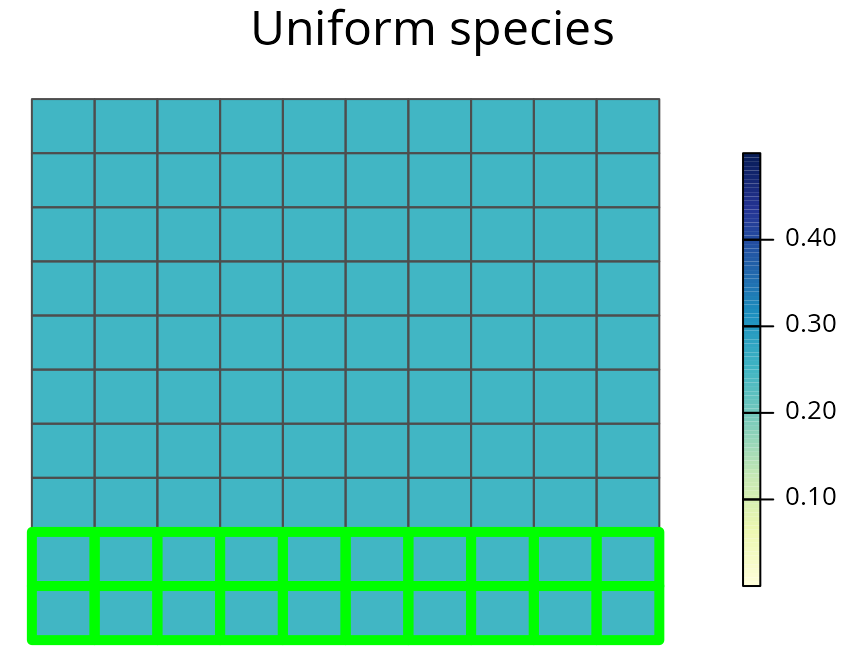
\includegraphics[width=3.5in,height=3.5in]{rapr_files/figure-latex/unnamed-chunk-12-1} 

}

\caption{A prioritisation for the uniformly distributed species generated using amount-based targets (20\%). Sqaures represent planning units. Planning units with a green border are selected for prioritisation, and their colour denotes the probability they are inhabited by the species.}\label{fig:unnamed-chunk-12}
\end{figure}

The prioritisation for the uniform species appears to be just a random
selection of planning units. This behavior is due to the fact that any
prioritisation with 20 planning units is optimal. By relying on just
amount targets, this solution may preserve a section of the species'
range core, or just focus on the range margin, or some random part of
its range--no emphasis is directed towards preserving different parts of
the species' range. This behavior highlights a fundamental limitation of
just using amount-based targets. In the absence of additional criteria,
conventional reserve selection problems do not contain any additional
information to identify the most effective prioritisation.

Now, we will generate a prioritisation for the normally distributed
species using amount-targets. We will use a similar process to what we
used for the uniformly distributed species, but for brevity, we will use
code to generate solutions immediately after updating the object.

\begin{Shaded}
\begin{Highlighting}[]
\CommentTok{# create new object with just the normal species}
\NormalTok{sim_ru_s2 <-}\StringTok{ }\KeywordTok{spp.subset}\NormalTok{(sim_ru, }\StringTok{'normal'}\NormalTok{)}
\end{Highlighting}
\end{Shaded}

\begin{Shaded}
\begin{Highlighting}[]
\CommentTok{# update amount targets to 20% and space targets to 0% and solve it}
\NormalTok{sim_rs_s2_amount <-}\StringTok{ }\KeywordTok{update}\NormalTok{(sim_ru_s2, }\DataTypeTok{amount.target=}\FloatTok{0.2}\NormalTok{, }\DataTypeTok{space.target=}\OtherTok{NA}\NormalTok{, }\DataTypeTok{solve=}\OtherTok{TRUE}\NormalTok{)}
\end{Highlighting}
\end{Shaded}

\begin{Shaded}
\begin{Highlighting}[]
\CommentTok{# show summary}
\KeywordTok{summary}\NormalTok{(sim_rs_s2_amount)}
\end{Highlighting}
\end{Shaded}

\begin{verbatim}
##   Run_Number Status Score Cost Planning_Units Connectivity_Total
## 1          1 MANUAL    10   10             10                220
##   Connectivity_In Connectivity_Edge Connectivity_Out
## 1              12               192               16
##   Connectivity_In_Fraction
## 1               0.05454545
\end{verbatim}

\begin{Shaded}
\begin{Highlighting}[]
\CommentTok{# show amount held}
\KeywordTok{amount.held}\NormalTok{(sim_rs_s2_amount)}
\end{Highlighting}
\end{Shaded}

\begin{verbatim}
##      normal
## 1 0.2026153
\end{verbatim}

\begin{Shaded}
\begin{Highlighting}[]
\CommentTok{# show space held}
\KeywordTok{space.held}\NormalTok{(sim_rs_s2_amount)}
\end{Highlighting}
\end{Shaded}

\begin{verbatim}
##   normal (Space 1)
## 1        0.6519926
\end{verbatim}

Now let's visualise the prioritisation we made for the normal species.

\begin{Shaded}
\begin{Highlighting}[]
\CommentTok{# plot the prioritisation and the normal species' distribution}
\KeywordTok{spp.plot}\NormalTok{(sim_rs_s2_amount, }\DecValTok{1}\NormalTok{, }\DataTypeTok{main=}\StringTok{'Normal species'}\NormalTok{)}
\end{Highlighting}
\end{Shaded}

\begin{figure}

{\centering 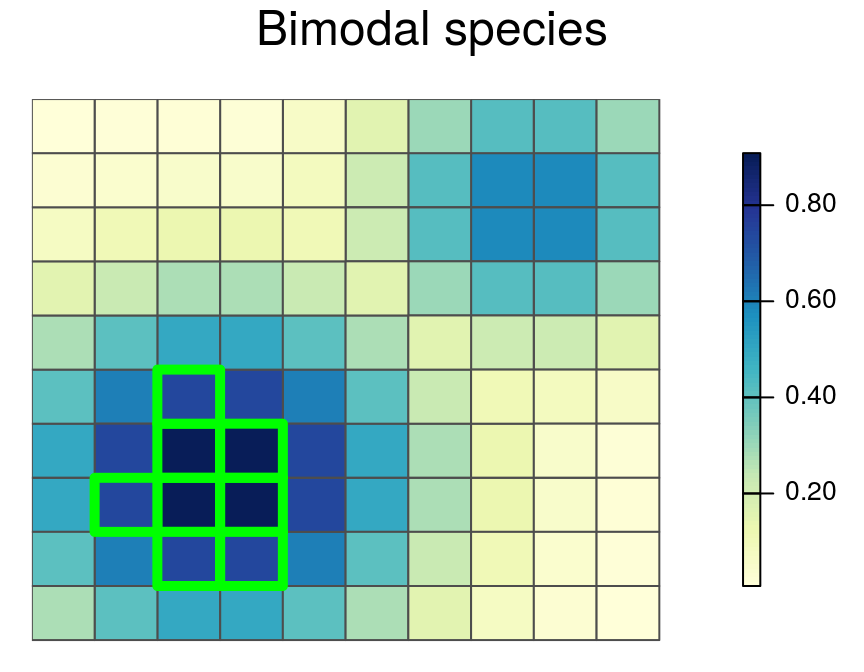
\includegraphics[width=3.5in,height=3.5in]{rapr_files/figure-latex/unnamed-chunk-17-1} 

}

\caption{A prioritisation for the normally distributed species generated using amount-based targets (20\%). See Figure 3 caption for conventions.}\label{fig:unnamed-chunk-17}
\end{figure}

The amount-based prioritisation for the normal species focuses only on
the species' range core. This prioritisation fails to secure any
peripheral parts of the species' distribution. As a consequence, it may
miss out on populations with novel adaptations to environmental
conditions along the species' range margin.

Now, let's generate an amount-based target for the bimodally distributed
species view it.

\begin{Shaded}
\begin{Highlighting}[]
\CommentTok{# create new object with just the bimodal species}
\NormalTok{sim_ru_s3 <-}\StringTok{ }\KeywordTok{spp.subset}\NormalTok{(sim_ru, }\StringTok{'bimodal'}\NormalTok{)}
\end{Highlighting}
\end{Shaded}

\begin{Shaded}
\begin{Highlighting}[]
\CommentTok{# update amount targets to 20% and space targets to 0% and solve it}
\NormalTok{sim_rs_s3_amount <-}\StringTok{ }\KeywordTok{update}\NormalTok{(sim_ru_s3, }\DataTypeTok{amount.target=}\FloatTok{0.2}\NormalTok{, }\DataTypeTok{space.target=}\OtherTok{NA}\NormalTok{)}
\end{Highlighting}
\end{Shaded}

\begin{Shaded}
\begin{Highlighting}[]
\CommentTok{# plot the prioritisation and the bimodal species' distribution}
\KeywordTok{spp.plot}\NormalTok{(sim_rs_s3_amount, }\DecValTok{1}\NormalTok{, }\DataTypeTok{main=}\StringTok{'Bimodal species'}\NormalTok{)}
\end{Highlighting}
\end{Shaded}

\begin{figure}

{\centering 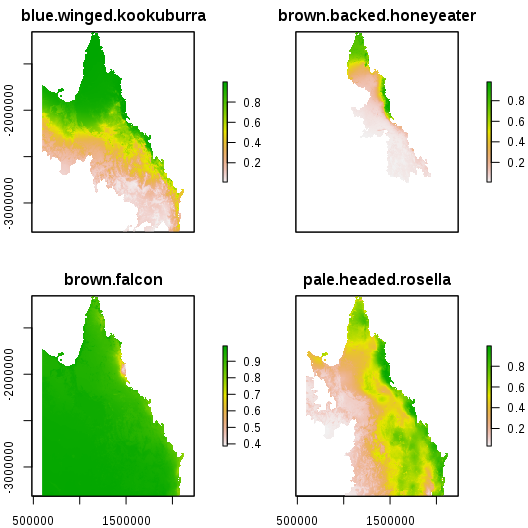
\includegraphics[width=3.5in,height=3.5in]{rapr_files/figure-latex/unnamed-chunk-21-1} 

}

\caption{A prioritisation for the bimodally distributed species generated using amount-based targets (20\%). See Figure 3 caption for conventions.}\label{fig:unnamed-chunk-21}
\end{figure}

\begin{Shaded}
\begin{Highlighting}[]
\CommentTok{# show summary}
\KeywordTok{summary}\NormalTok{(sim_rs_s3_amount)}
\end{Highlighting}
\end{Shaded}

\begin{verbatim}
##   Run_Number Status Score Cost Planning_Units Connectivity_Total
## 1          1 MANUAL     8    8              8                220
##   Connectivity_In Connectivity_Edge Connectivity_Out
## 1               9               197               14
##   Connectivity_In_Fraction
## 1               0.04090909
\end{verbatim}

\begin{Shaded}
\begin{Highlighting}[]
\CommentTok{# show amount held}
\KeywordTok{amount.held}\NormalTok{(sim_rs_s3_amount)}
\end{Highlighting}
\end{Shaded}

\begin{verbatim}
##     bimodal
## 1 0.2018391
\end{verbatim}

\begin{Shaded}
\begin{Highlighting}[]
\CommentTok{# show space held}
\KeywordTok{space.held}\NormalTok{(sim_rs_s3_amount)}
\end{Highlighting}
\end{Shaded}

\begin{verbatim}
##   bimodal (Space 1)
## 1         0.2829105
\end{verbatim}

The amount-based prioritisation for the bimodally distributed species
only selects planning units in the bottom left corner of the study area.
This prioritisation only preserves individuals belonging to one of the
two ecotypes. As a consequence, this prioritisation may fail to preserve
a representative sample of the genetic variation found inside this
species.

\subparagraph{Amount-based and space-based
targets}\label{amount-based-and-space-based-targets}

Now that we have generated a prioritisation for each species using only
amount-based targets, we will generate a prioritisations using both
amount-based and space-targets. To do this we will update the space
targets in our amount-based prioritisations to 50\%, and store the new
prioritisations in new objects.

First, let's do this for the uniform species.

\begin{Shaded}
\begin{Highlighting}[]
\CommentTok{# make new prioritisation}
\NormalTok{sim_rs_s1_space <-}\StringTok{ }\KeywordTok{update}\NormalTok{(sim_rs_s1_amount, }\DataTypeTok{amount.target=}\FloatTok{0.2}\NormalTok{, }\DataTypeTok{space.target=}\FloatTok{0.5}\NormalTok{)}
\end{Highlighting}
\end{Shaded}

\begin{Shaded}
\begin{Highlighting}[]
\CommentTok{# show summary}
\KeywordTok{summary}\NormalTok{(sim_rs_s1_space)}
\end{Highlighting}
\end{Shaded}

\begin{verbatim}
##   Run_Number Status Score Cost Planning_Units Connectivity_Total
## 1          1 MANUAL    20   20             20                220
##   Connectivity_In Connectivity_Edge Connectivity_Out
## 1              18               147               55
##   Connectivity_In_Fraction
## 1               0.08181818
\end{verbatim}

\begin{Shaded}
\begin{Highlighting}[]
\CommentTok{# show amount held}
\KeywordTok{amount.held}\NormalTok{(sim_rs_s1_space)}
\end{Highlighting}
\end{Shaded}

\begin{verbatim}
##   uniform
## 1     0.2
\end{verbatim}

\begin{Shaded}
\begin{Highlighting}[]
\CommentTok{# show space held}
\KeywordTok{space.held}\NormalTok{(sim_rs_s1_space)}
\end{Highlighting}
\end{Shaded}

\begin{verbatim}
##   uniform (Space 1)
## 1         0.8793939
\end{verbatim}

Let's take a look at the prioritisation for the uniform species with
amount-based and space-based targets. Then, let's compare the solutions
for the amount-based prioritisation with the new prioritisation using
both amount and space targets.

\begin{Shaded}
\begin{Highlighting}[]
\CommentTok{# plot the prioritisation and the uniform species' distribution}
\KeywordTok{spp.plot}\NormalTok{(sim_rs_s1_space, }\StringTok{'uniform'}\NormalTok{, }\DataTypeTok{main=}\StringTok{'Uniform species'}\NormalTok{)}
\end{Highlighting}
\end{Shaded}

\begin{figure}

{\centering 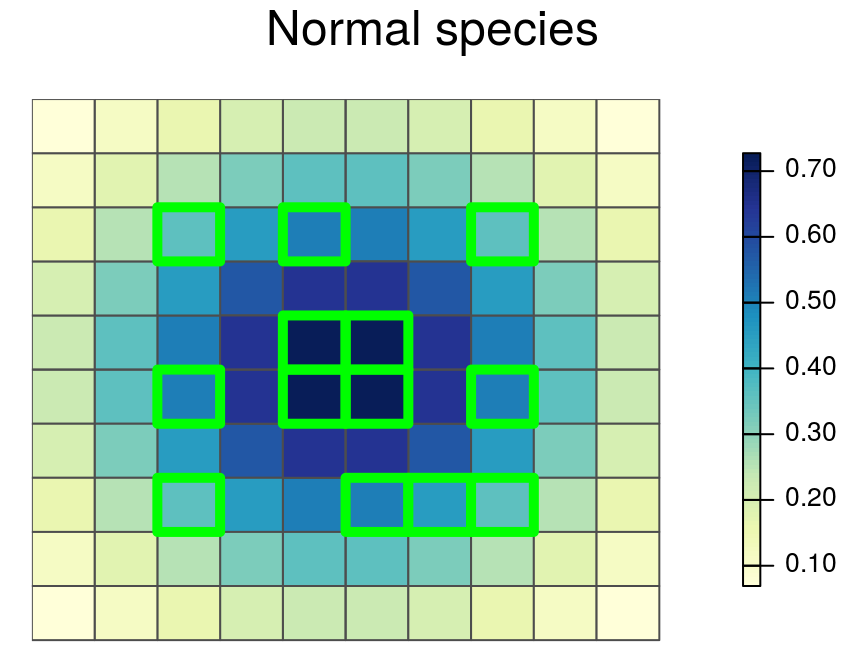
\includegraphics[width=3.5in,height=3.5in]{rapr_files/figure-latex/unnamed-chunk-26-1} 

}

\caption{A prioritisation for the uniformly distributed species generated using amount-based targets (20\%) and space-based targets (85\%). See Figure 3 caption for conventions.}\label{fig:unnamed-chunk-26}
\end{figure}

\begin{Shaded}
\begin{Highlighting}[]
\CommentTok{# plot the difference between old and new prioritisations}
\KeywordTok{plot}\NormalTok{(sim_rs_s1_amount, sim_rs_s1_space, }\DecValTok{1}\NormalTok{, }\DecValTok{1}\NormalTok{, }\DataTypeTok{main=}\StringTok{'Difference between solutions'}\NormalTok{)}
\end{Highlighting}
\end{Shaded}

\begin{figure}

{\centering 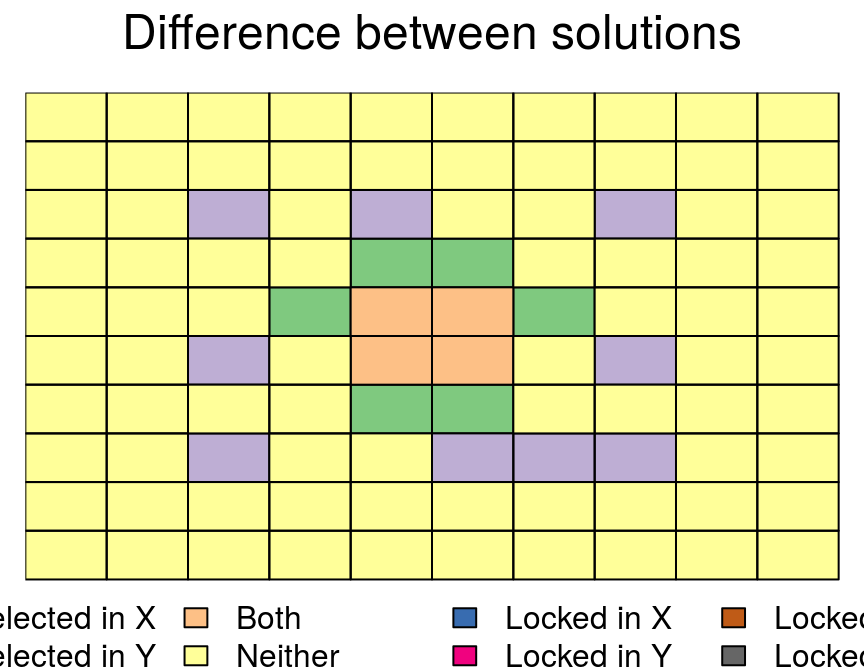
\includegraphics[width=3.5in,height=3.5in]{rapr_files/figure-latex/unnamed-chunk-27-1} 

}

\caption{Difference between two prioritisations for the uniformly distributed species. Prioritisation $X$ was generated using just amount-based targets (20\%), and prioritisation $Y$ was generated using an additional space-based target (85\%).}\label{fig:unnamed-chunk-27}
\end{figure}

Here we can see that by including a space-target, the prioritisation is
spread out evenly across the species' distribution. Unlike the
amount-based prioritisation, this prioritisation samples all the
different parts of the species' distribution.

Now, let's generate a prioritisation for the normally distributed
species that considers amount-based and space-based targets. Then, let's
visualise the new prioritisation and compare it to the old amount-based
prioritisation.

\begin{Shaded}
\begin{Highlighting}[]
\CommentTok{# make new prioritisation}
\NormalTok{sim_rs_s2_space <-}\StringTok{ }\KeywordTok{update}\NormalTok{(sim_rs_s2_amount, }\DataTypeTok{amount.target=}\FloatTok{0.2}\NormalTok{, }\DataTypeTok{space.target=}\FloatTok{0.85}\NormalTok{)}
\end{Highlighting}
\end{Shaded}

\begin{Shaded}
\begin{Highlighting}[]
\CommentTok{# show summary}
\KeywordTok{summary}\NormalTok{(sim_rs_s2_space)}
\end{Highlighting}
\end{Shaded}

\begin{verbatim}
##   Run_Number Status Score Cost Planning_Units Connectivity_Total
## 1          1 MANUAL    13   13             13                220
##   Connectivity_In Connectivity_Edge Connectivity_Out
## 1               7               175               38
##   Connectivity_In_Fraction
## 1               0.03181818
\end{verbatim}

\begin{Shaded}
\begin{Highlighting}[]
\CommentTok{# show amount held}
\KeywordTok{amount.held}\NormalTok{(sim_rs_s2_space)}
\end{Highlighting}
\end{Shaded}

\begin{verbatim}
##      normal
## 1 0.2122983
\end{verbatim}

\begin{Shaded}
\begin{Highlighting}[]
\CommentTok{# show space held}
\KeywordTok{space.held}\NormalTok{(sim_rs_s2_space)}
\end{Highlighting}
\end{Shaded}

\begin{verbatim}
##   normal (Space 1)
## 1        0.8523318
\end{verbatim}

\begin{Shaded}
\begin{Highlighting}[]
\CommentTok{# plot the prioritisation and the normal species' distribution}
\KeywordTok{spp.plot}\NormalTok{(sim_rs_s2_space, }\StringTok{'normal'}\NormalTok{, }\DataTypeTok{main=}\StringTok{'Normal species'}\NormalTok{)}
\end{Highlighting}
\end{Shaded}

\begin{figure}

{\centering 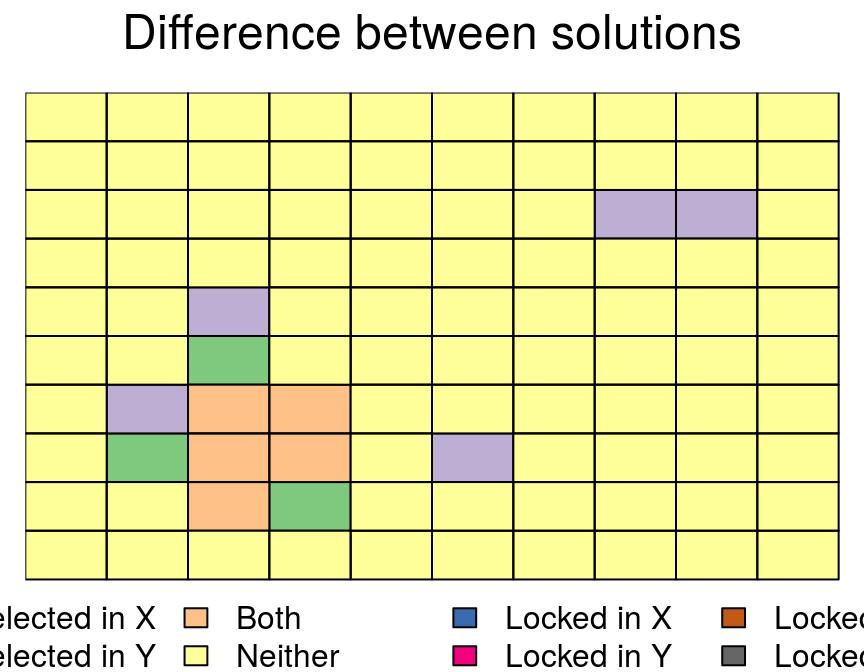
\includegraphics[width=3.5in,height=3.5in]{rapr_files/figure-latex/unnamed-chunk-31-1} 

}

\caption{A prioritisation for the normally distributed species generated using amount-based targets (20\%) and space-based targets (85\%). See Figure 3 caption for conventions.}\label{fig:unnamed-chunk-31}
\end{figure}

\begin{Shaded}
\begin{Highlighting}[]
\CommentTok{# plot the difference between old and new prioritisations}
\KeywordTok{plot}\NormalTok{(sim_rs_s2_amount, sim_rs_s2_space, }\DecValTok{1}\NormalTok{, }\DecValTok{1}\NormalTok{, }\DataTypeTok{main=}\StringTok{'Difference between solutions'}\NormalTok{)}
\end{Highlighting}
\end{Shaded}

\begin{figure}

{\centering 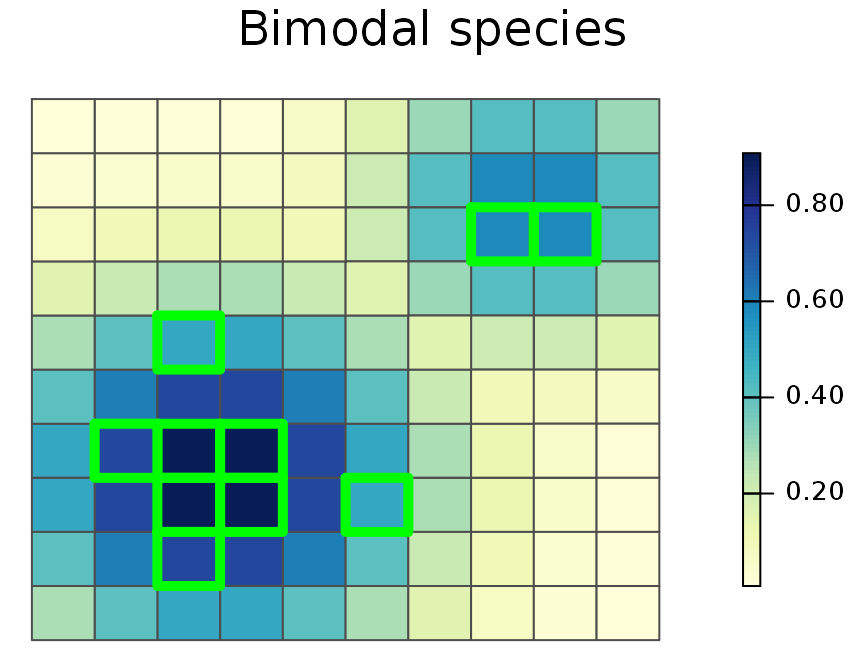
\includegraphics[width=3.5in,height=3.5in]{rapr_files/figure-latex/unnamed-chunk-32-1} 

}

\caption{Difference between two prioritisations for the normally distributed species. See Figure 7 caption for conventions.}\label{fig:unnamed-chunk-32}
\end{figure}

We can see by using both amount-based and space-based targets we can
obtain a prioritisation that secures both the species' range core and
parts of its range margin. As a consequence, it may capture any novel
adaptations found along the species' range margin--unlike the
amount-based prioritisation.

Finally, let's generate a prioritisation for the bimodal species using
amount-based and space-based targets.

\begin{Shaded}
\begin{Highlighting}[]
\CommentTok{# make new prioritisation}
\NormalTok{sim_rs_s3_space <-}\StringTok{ }\KeywordTok{update}\NormalTok{(sim_rs_s3_amount, }\DataTypeTok{amount.target=}\FloatTok{0.2}\NormalTok{, }\DataTypeTok{space.target=}\FloatTok{0.85}\NormalTok{)}
\end{Highlighting}
\end{Shaded}

\begin{Shaded}
\begin{Highlighting}[]
\CommentTok{# show summary}
\KeywordTok{summary}\NormalTok{(sim_rs_s3_space)}
\end{Highlighting}
\end{Shaded}

\begin{verbatim}
##   Run_Number Status Score Cost Planning_Units Connectivity_Total
## 1          1 MANUAL     9    9              9                220
##   Connectivity_In Connectivity_Edge Connectivity_Out
## 1               9               193               18
##   Connectivity_In_Fraction
## 1               0.04090909
\end{verbatim}

\begin{Shaded}
\begin{Highlighting}[]
\CommentTok{# show amount held}
\KeywordTok{amount.held}\NormalTok{(sim_rs_s3_space)}
\end{Highlighting}
\end{Shaded}

\begin{verbatim}
##    bimodal
## 1 0.219729
\end{verbatim}

\begin{Shaded}
\begin{Highlighting}[]
\CommentTok{# show space held}
\KeywordTok{space.held}\NormalTok{(sim_rs_s3_space)}
\end{Highlighting}
\end{Shaded}

\begin{verbatim}
##   bimodal (Space 1)
## 1         0.8813757
\end{verbatim}

\begin{Shaded}
\begin{Highlighting}[]
\CommentTok{# plot the prioritisation and the bimodal species' distribution}
\KeywordTok{spp.plot}\NormalTok{(sim_rs_s3_space, }\StringTok{'bimodal'}\NormalTok{, }\DataTypeTok{main=}\StringTok{'Bimodal species'}\NormalTok{)}
\end{Highlighting}
\end{Shaded}

\begin{figure}

{\centering 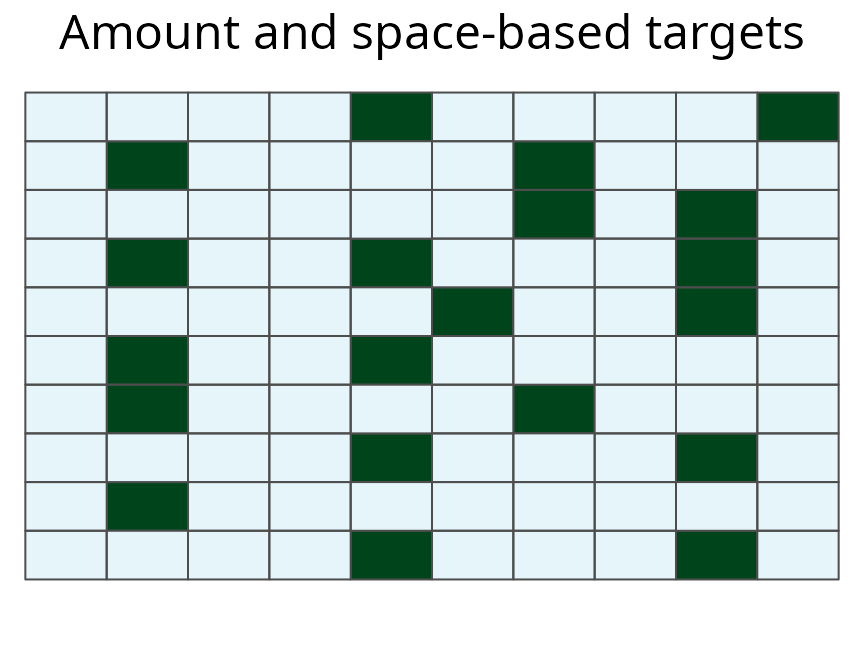
\includegraphics[width=3.5in,height=3.5in]{rapr_files/figure-latex/unnamed-chunk-36-1} 

}

\caption{A prioritisation for the normally distributed species generated using amount-based targets (20\%) and space-based targets (85\%). See Figure 3 caption for conventions.}\label{fig:unnamed-chunk-36}
\end{figure}

\begin{Shaded}
\begin{Highlighting}[]
\CommentTok{# plot the difference between old and new prioritisations}
\KeywordTok{plot}\NormalTok{(sim_rs_s3_amount, sim_rs_s3_space, }\DecValTok{1}\NormalTok{, }\DecValTok{1}\NormalTok{, }\DataTypeTok{main=}\StringTok{'Difference between solutions'}\NormalTok{)}
\end{Highlighting}
\end{Shaded}

\begin{figure}

{\centering 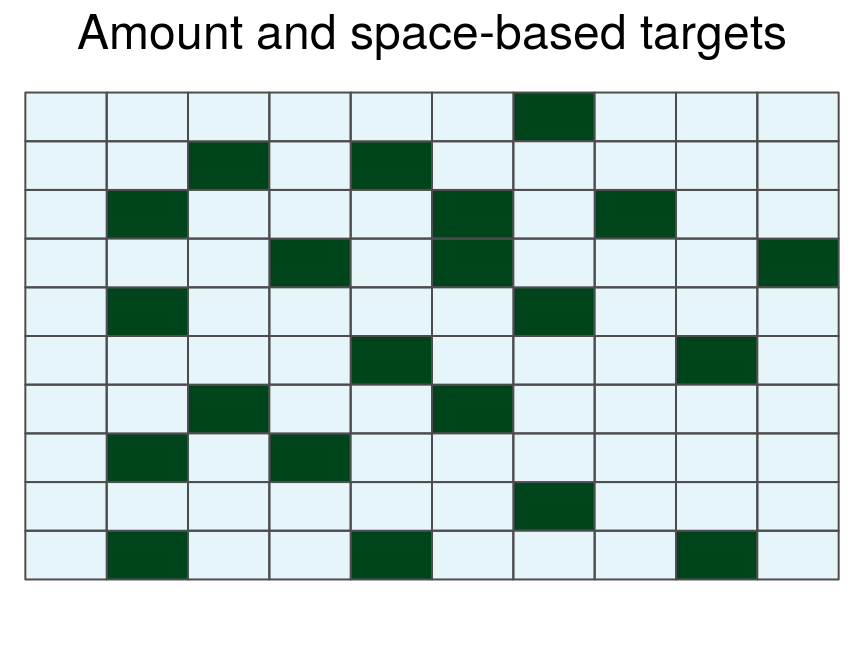
\includegraphics[width=3.5in,height=3.5in]{rapr_files/figure-latex/unnamed-chunk-37-1} 

}

\caption{Difference between two prioritisations for the bimodally distributed species. See Figure 7 caption for conventions.}\label{fig:unnamed-chunk-37}
\end{figure}

Earlier we found that the amount-based prioritisation only preserved
individuals from a single ecotype, and would have failed to adequately
preserve the intra-specific variation for this species. However, here we
can see that by including space-based targets, we can develop
prioritisations that secure individuals belonging to both ecotypes. This
new prioritisation is much more effective at sampling the intra-specific
variation for this species.

Overall, these results demonstrate that under the simplest of
conditions, the use of space-based targets can improve prioritisations.
However, these prioritisations were each generated for a single species.
It is possible that prioritisations generated using multiple species may
do a better job at preserving the intra-specific variation for
individuals species by preserving them in different parts of their
range. We will investigate this in the next section.

\paragraph{Multi-species
prioritisations}\label{multi-species-prioritisations}

\subparagraph{Effects of including space-based
targets}\label{effects-of-including-space-based-targets}

So far we have generated prioritisations using only a single species at
a time. However, real world prioritisations are often generated using
multiple species to ensure that they preserve a comprehensive set of
biodiversity. Here, we will generate multi-species prioritisations that
preserve all three of the simulated species. First, we will generate a
prioritisation using amount-based targets that only aims to preserve
20\% of the area they occupy. Then, we will generate a prioritisation
that also incoperate space-based targets to also preserve 85\% of their
geographic distribution. We will then compare the two prioritisations.

\begin{Shaded}
\begin{Highlighting}[]
\CommentTok{# make prioritisations}
\NormalTok{sim_mrs_amount <-}\StringTok{ }\KeywordTok{update}\NormalTok{(}
    \NormalTok{sim_ru,}
    \DataTypeTok{amount.target=}\KeywordTok{c}\NormalTok{(}\FloatTok{0.2}\NormalTok{,}\FloatTok{0.2}\NormalTok{,}\FloatTok{0.2}\NormalTok{),}
    \DataTypeTok{space.target=}\KeywordTok{c}\NormalTok{(}\DecValTok{0}\NormalTok{,}\DecValTok{0}\NormalTok{,}\DecValTok{0}\NormalTok{)}
\NormalTok{)}

\NormalTok{sim_mrs_space <-}\StringTok{ }\KeywordTok{update}\NormalTok{(}
    \NormalTok{sim_ru,}
    \DataTypeTok{amount.target=}\KeywordTok{c}\NormalTok{(}\FloatTok{0.2}\NormalTok{,}\FloatTok{0.2}\NormalTok{,}\FloatTok{0.2}\NormalTok{),}
    \DataTypeTok{space.target=}\KeywordTok{c}\NormalTok{(}\FloatTok{0.85}\NormalTok{, }\FloatTok{0.85}\NormalTok{, }\FloatTok{0.85}\NormalTok{)}
\NormalTok{)}
\end{Highlighting}
\end{Shaded}

\begin{Shaded}
\begin{Highlighting}[]
\CommentTok{# show summaries}
\KeywordTok{summary}\NormalTok{(sim_mrs_amount)}
\end{Highlighting}
\end{Shaded}

\begin{verbatim}
##   Run_Number Status Score Cost Planning_Units Connectivity_Total
## 1          1 MANUAL    20   20             20                220
##   Connectivity_In Connectivity_Edge Connectivity_Out
## 1              17               147               56
##   Connectivity_In_Fraction
## 1               0.07727273
\end{verbatim}

\begin{Shaded}
\begin{Highlighting}[]
\KeywordTok{summary}\NormalTok{(sim_mrs_space)}
\end{Highlighting}
\end{Shaded}

\begin{verbatim}
##   Run_Number Status Score Cost Planning_Units Connectivity_Total
## 1          1 MANUAL    20   20             20                220
##   Connectivity_In Connectivity_Edge Connectivity_Out
## 1               7               142               71
##   Connectivity_In_Fraction
## 1               0.03181818
\end{verbatim}

\begin{Shaded}
\begin{Highlighting}[]
\CommentTok{# show amount held for each prioritisation}
\KeywordTok{amount.held}\NormalTok{(sim_mrs_amount)}
\end{Highlighting}
\end{Shaded}

\begin{verbatim}
##   uniform   normal   bimodal
## 1     0.2 0.201559 0.2012952
\end{verbatim}

\begin{Shaded}
\begin{Highlighting}[]
\KeywordTok{amount.held}\NormalTok{(sim_mrs_space)}
\end{Highlighting}
\end{Shaded}

\begin{verbatim}
##   uniform    normal   bimodal
## 1     0.2 0.2185579 0.2232897
\end{verbatim}

\begin{Shaded}
\begin{Highlighting}[]
\CommentTok{# show space held for each prioritisation}
\KeywordTok{space.held}\NormalTok{(sim_mrs_amount)}
\end{Highlighting}
\end{Shaded}

\begin{verbatim}
##   uniform (Space 1) normal (Space 1) bimodal (Space 1)
## 1         0.8593939        0.8205165         0.8866593
\end{verbatim}

\begin{Shaded}
\begin{Highlighting}[]
\KeywordTok{space.held}\NormalTok{(sim_mrs_space)}
\end{Highlighting}
\end{Shaded}

\begin{verbatim}
##   uniform (Space 1) normal (Space 1) bimodal (Space 1)
## 1         0.9321212        0.8805152         0.9261063
\end{verbatim}

\begin{Shaded}
\begin{Highlighting}[]
\CommentTok{# plot multi-species prioritisation with amount-based targets}
\KeywordTok{plot}\NormalTok{(sim_mrs_amount, }\DecValTok{1}\NormalTok{, }\DataTypeTok{main=}\StringTok{'Amount-based targets'}\NormalTok{)}
\end{Highlighting}
\end{Shaded}

\begin{figure}

{\centering 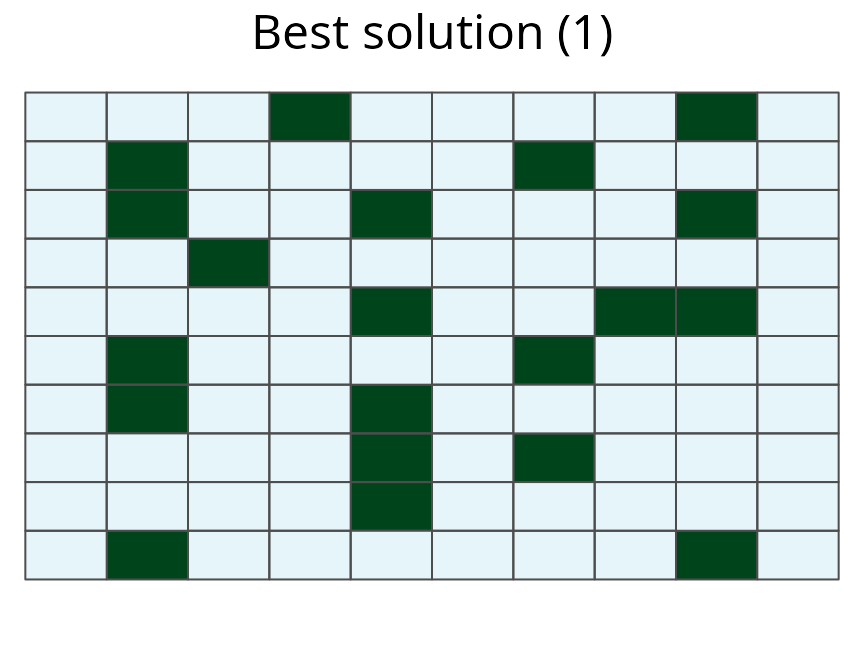
\includegraphics[width=3.5in,height=3.5in]{rapr_files/figure-latex/unnamed-chunk-41-1} 

}

\caption{A multi-species prioritisation for the uniformly, normally, and bimodally distributed species generated using just amount-based targets (20\%). Squares represent planning units. Dark green planning units are selected for preservation.}\label{fig:unnamed-chunk-41}
\end{figure}

\begin{Shaded}
\begin{Highlighting}[]
\CommentTok{# plot multi-species prioritisation with amount- and space-based targets}
\KeywordTok{plot}\NormalTok{(sim_mrs_space, }\DecValTok{1}\NormalTok{, }\DataTypeTok{main=}\StringTok{'Amount and space-based targets'}\NormalTok{)}
\end{Highlighting}
\end{Shaded}

\begin{figure}

{\centering 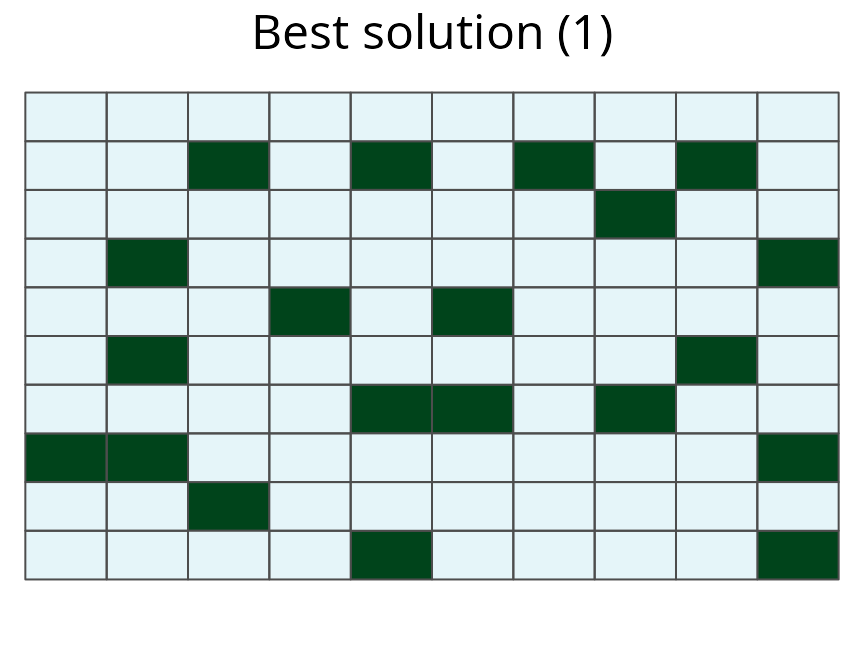
\includegraphics[width=3.5in,height=3.5in]{rapr_files/figure-latex/unnamed-chunk-42-1} 

}

\caption{A multi-species prioritisation for the uniformly, normally, and bimodally distributed species generated using amount-based targets (20\%) and space-based targets (85\%). See Figure 12 caption for conventions.}\label{fig:unnamed-chunk-42}
\end{figure}

\begin{Shaded}
\begin{Highlighting}[]
\CommentTok{# difference between the two prioritisations}
\KeywordTok{plot}\NormalTok{(sim_mrs_amount, sim_mrs_space, }\DecValTok{1}\NormalTok{, }\DecValTok{1}\NormalTok{, }\DataTypeTok{main=}\StringTok{'Difference between solutions'}\NormalTok{)}
\end{Highlighting}
\end{Shaded}

\begin{figure}

{\centering 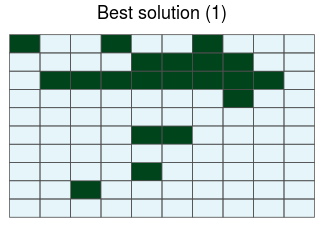
\includegraphics[width=3.5in,height=3.5in]{rapr_files/figure-latex/unnamed-chunk-43-1} 

}

\caption{Difference between two multi-species prioritisations. See Figure 7 caption for conventions.}\label{fig:unnamed-chunk-43}
\end{figure}

Here we can see that the inclusion of space-based targets changes which
planning units are selected for prioritisation, but also the number of
planning units that are selected. The amount-based prioritisation is
comprised of 20 units, and the space-based prioritisation is comprised
of 20 units. This result suggests that an adequate and representative
prioritisation can be achieved for only a minor increase in cost.

\subparagraph{Uncertainty in species'
distributions}\label{uncertainty-in-species-distributions}

The unreliable formulation does not consider the probability that the
planning units are occupied by features when calculating how well a
given solution secures a representative sample of an attribute space.
Thus solutions identified using the unreliable formulation may select
regions of an attribute space for a species using planning units that
only have a small chance of being inhabited. As a consequence, if the
prioritisation is implemented, it may fail to secure regions of an
attribute space if individuals do not inhabit these planning units, and
ultimately fail to fulfil the space-based targets.

A simple solution to this issue would be to ensure that planning units
cannot be assigned to demand points if they have a low probability of
occupancy. This can be achieved by setting a probability threshold for
planning units, such that planning units with a probability of occupancy
below the threshold are effectively set to zero.

\begin{Shaded}
\begin{Highlighting}[]
\CommentTok{# make new prioritisation with probability threshold of 0.5 for each species}
\NormalTok{sim_mrs_space2 <-}\StringTok{ }\KeywordTok{solve}\NormalTok{(}
    \KeywordTok{prob.subset}\NormalTok{(}
        \NormalTok{sim_mrs_space,}
        \DataTypeTok{species=}\DecValTok{1}\NormalTok{:}\DecValTok{3}\NormalTok{,}
        \DataTypeTok{threshold=}\KeywordTok{c}\NormalTok{(}\FloatTok{0.1}\NormalTok{,}\FloatTok{0.1}\NormalTok{,}\FloatTok{0.1}\NormalTok{)}
    \NormalTok{)}
\NormalTok{)}
\end{Highlighting}
\end{Shaded}

\begin{Shaded}
\begin{Highlighting}[]
\CommentTok{# show summary}
\KeywordTok{summary}\NormalTok{(sim_mrs_space2)}
\end{Highlighting}
\end{Shaded}

\begin{verbatim}
##   Run_Number Status Score Cost Planning_Units Connectivity_Total
## 1          1 MANUAL    20   20             20                220
##   Connectivity_In Connectivity_Edge Connectivity_Out
## 1               7               143               70
##   Connectivity_In_Fraction
## 1               0.03181818
\end{verbatim}

\begin{Shaded}
\begin{Highlighting}[]
\CommentTok{# plot prioritisation}
\KeywordTok{plot}\NormalTok{(sim_mrs_space2, }\DecValTok{1}\NormalTok{)}
\end{Highlighting}
\end{Shaded}

\begin{figure}

{\centering 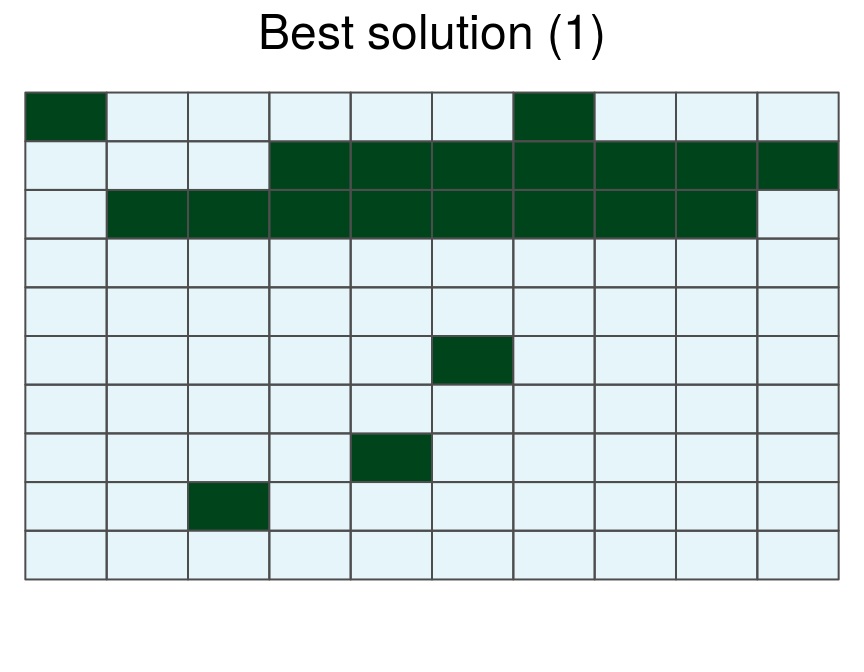
\includegraphics[width=3.5in,height=3.5in]{rapr_files/figure-latex/unnamed-chunk-47-1} 

}

\caption{A multi-species prioritisation for the uniformly, normally, and bimodally distributed species generated using amount-based targets (20\%) and space-based targets (85\%). This priorititisation was generated to be robust against low occupancy probabilities, by preventing planning units with low probabilities from being used to represent demand points. See Figure 12 caption for conventions.}\label{fig:unnamed-chunk-47}
\end{figure}

\begin{Shaded}
\begin{Highlighting}[]
\CommentTok{# difference between prioritisations that use and do not use thresholds}
\KeywordTok{plot}\NormalTok{(sim_mrs_space2, sim_mrs_space, }\DecValTok{1}\NormalTok{, }\DecValTok{1}\NormalTok{, }\DataTypeTok{main=}\StringTok{'Difference between solutions'}\NormalTok{)}
\end{Highlighting}
\end{Shaded}

\begin{figure}

{\centering 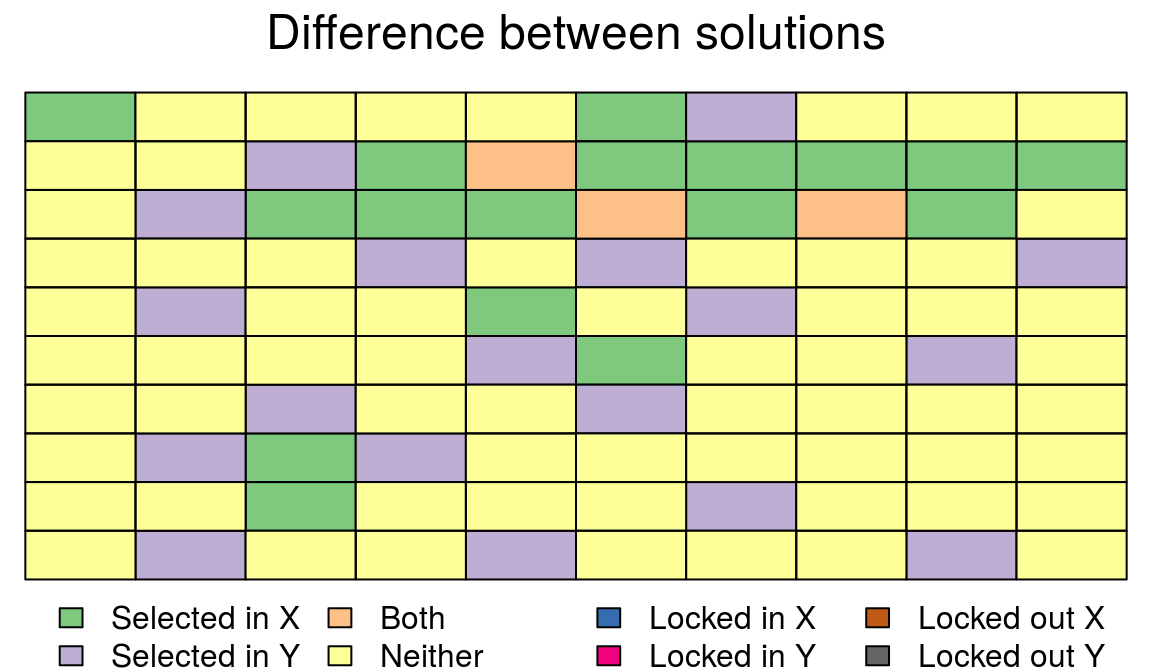
\includegraphics[width=3.5in,height=3.5in]{rapr_files/figure-latex/unnamed-chunk-48-1} 

}

\caption{Difference between two multi-species prioritisations. See Figure 7 caption for conventions.}\label{fig:unnamed-chunk-48}
\end{figure}

But this method requires setting somewhat arbitrary thresholds. A more
robust solution to this issue is to actually use the probability that
species occupy planning units to generate the prioritisations. This is
what the reliable formulation does. First we will try and generate a
solution using existing targets and the reliable formulation. To reduce
computational time, we will set the maximum backup $R$-level to 1.

\begin{Shaded}
\begin{Highlighting}[]
\CommentTok{# make new prioritisation using reliable formulation}
\NormalTok{sim_mrs_space3 <-}\StringTok{ }\KeywordTok{try}\NormalTok{(}\KeywordTok{update}\NormalTok{(sim_mrs_space, }\DataTypeTok{formulation=}\StringTok{'reliable'}\NormalTok{, }\DataTypeTok{max.r.level=}\NormalTok{1L))}
\end{Highlighting}
\end{Shaded}

\begin{verbatim}
## Warning for adding variables: zero or small (< 1e-13) coefficients, ignored
## Optimize a model with 364206 rows, 181900 columns and 3847200 nonzeros
## Coefficient statistics:
##   Matrix range    [6e-05, 1e+02]
##   Objective range [1e+00, 1e+00]
##   Bounds range    [1e+00, 1e+00]
##   RHS range       [7e-03, 6e+01]
## Presolve removed 349813 rows and 90706 columns
## Presolve time: 3.98s
## 
## Explored 0 nodes (0 simplex iterations) in 6.76 seconds
## Thread count was 1 (of 2 available processors)
## 
## Model is infeasible
## Best objective -, best bound -, gap -
## Try setting lower space-based targets.
##  Below are the maximum targets for each species and space.
##   Proportion            Target
## 1   -1.97000 uniform (Space 1)
## 2  -12.67570  normal (Space 1)
## 3  -21.69092 bimodal (Space 1)
\end{verbatim}

However, this fails. The reason why we cannot generate a prioritisation
is because we require more planning units to generate a solution that
fulfills the targets when we consider probabilities. This is confirmed
by the negative maximum targets shown in the error message. Now, we will
set lower targets and generate solution.

\begin{Shaded}
\begin{Highlighting}[]
\CommentTok{# make new prioritisation using reliable formulation and reduced targets}
\NormalTok{sim_mrs_space3 <-}\StringTok{ }\KeywordTok{update}\NormalTok{(}
    \NormalTok{sim_mrs_space,}
    \DataTypeTok{formulation=}\StringTok{'reliable'}\NormalTok{,}
    \DataTypeTok{max.r.level=}\NormalTok{1L,}
    \DataTypeTok{space.target=}\NormalTok{-}\DecValTok{25}
\NormalTok{)}
\end{Highlighting}
\end{Shaded}

\begin{Shaded}
\begin{Highlighting}[]
\CommentTok{# show summary}
\KeywordTok{summary}\NormalTok{(sim_mrs_space3)}
\end{Highlighting}
\end{Shaded}

\begin{verbatim}
##   Run_Number Status Score Cost Planning_Units Connectivity_Total
## 1          1 MANUAL    20   20             20                220
##   Connectivity_In Connectivity_Edge Connectivity_Out
## 1              28               161               31
##   Connectivity_In_Fraction
## 1                0.1272727
\end{verbatim}

\begin{Shaded}
\begin{Highlighting}[]
\CommentTok{# plot prioritisation}
\KeywordTok{plot}\NormalTok{(sim_mrs_space3, }\DecValTok{1}\NormalTok{)}
\end{Highlighting}
\end{Shaded}

\begin{figure}

{\centering 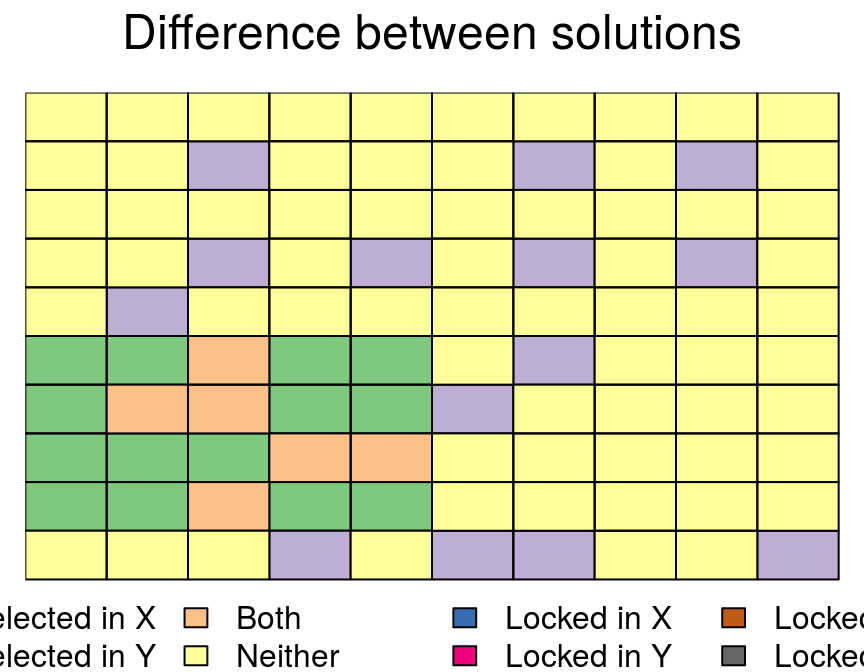
\includegraphics[width=3.5in,height=3.5in]{rapr_files/figure-latex/unnamed-chunk-53-1} 

}

\caption{A multi-species prioritisation for the uniformly, normally, and bimodally distributed species generated using amount-based targets (20\%) and space-based targets (85\%). This priorititisation was generated to be robust against low occupancy probabilities, by explicitly using the probability of occupancy data when deriving a solution. See Figure 12 caption for conventions.}\label{fig:unnamed-chunk-53}
\end{figure}

\begin{Shaded}
\begin{Highlighting}[]
\CommentTok{# difference between prioritisations based on unreliable and reliable formulation}
\KeywordTok{plot}\NormalTok{(sim_mrs_space3, sim_mrs_space, }\DecValTok{1}\NormalTok{, }\DecValTok{1}\NormalTok{, }\DataTypeTok{main=}\StringTok{'Difference between solutions'}\NormalTok{)}
\end{Highlighting}
\end{Shaded}

\begin{figure}

{\centering 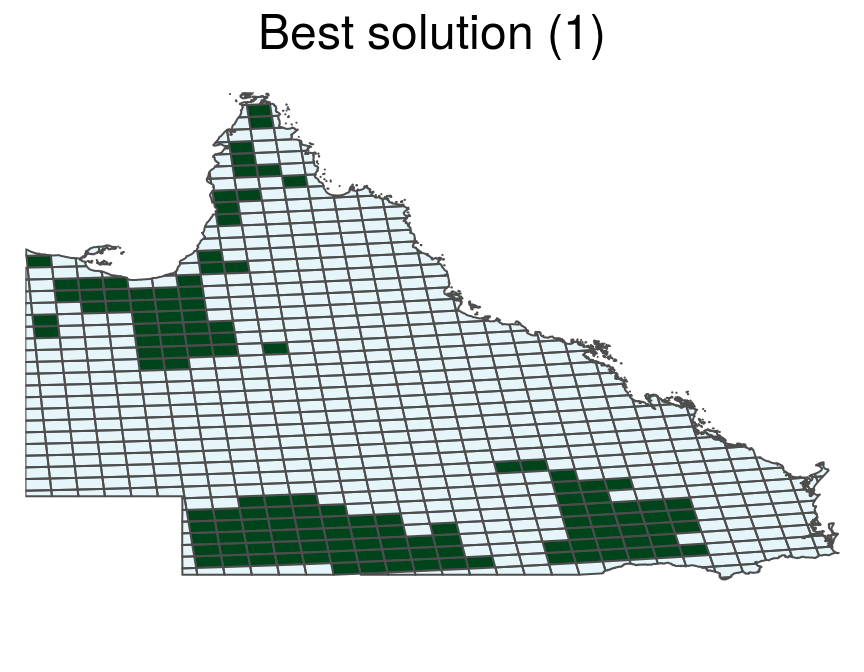
\includegraphics[width=3.5in,height=3.5in]{rapr_files/figure-latex/unnamed-chunk-54-1} 

}

\caption{Difference between two multi-species prioritisations. See Figure 7 caption for conventions.}\label{fig:unnamed-chunk-54}
\end{figure}

An additional planning unit was selected using the reliable formulation.
The prioritisation based on the unreliable formulation had 20 planning
units, but the prioritisation based on the reliable formlation has 20
planning units. This differnce occurs because the reliable formulation
needs to ensure that all selected planning units with a low chance of
being occupied have a suitable backup planning unit. While the reliable
formulation can deliver more robust prioritisations, it takes much
longer to solve conservation planning problems expressed using this
formulation than the unreliable formulation. As a consequence, the
reliable formulation is only feasible for particularly small problems,
such as those involving few features and less than several hundred
planning units.

\subparagraph{Fragmentation}\label{fragmentation}

Fragmentation is an important consideration in real-world planning
situations. Up until now, we haven't considered the effects of
fragmentation on the viability of the prioritisation. As a consequence,
our prioritisations have tended to contain planning units without any
neighbours. We can use the \texttt{BLM} parameter to penalise fragmented
solutions.

Let's generate a new prioritisation that heavily penalises
fragmentation. Here, we will update the \texttt{sim\_mrs\_amount} object
with \texttt{BLM} of 100.

\begin{Shaded}
\begin{Highlighting}[]
\CommentTok{# update prioritisation}
\NormalTok{sim_mrs_amount_blm <-}\StringTok{ }\KeywordTok{update}\NormalTok{(sim_mrs_amount, }\DataTypeTok{BLM=}\DecValTok{100}\NormalTok{)}
\end{Highlighting}
\end{Shaded}

\begin{Shaded}
\begin{Highlighting}[]
\CommentTok{# show summary of prioritisation}
\KeywordTok{summary}\NormalTok{(sim_mrs_amount_blm)}
\end{Highlighting}
\end{Shaded}

\begin{verbatim}
##   Run_Number Status Score Cost Planning_Units Connectivity_Total
## 1          1 MANUAL  1420   20             20                220
##   Connectivity_In Connectivity_Edge Connectivity_Out
## 1              35               171               14
##   Connectivity_In_Fraction
## 1                0.1590909
\end{verbatim}

\begin{Shaded}
\begin{Highlighting}[]
\CommentTok{# show amount held for each prioritisation}
\KeywordTok{amount.held}\NormalTok{(sim_mrs_amount_blm)}
\end{Highlighting}
\end{Shaded}

\begin{verbatim}
##   uniform    normal   bimodal
## 1     0.2 0.2645832 0.3911267
\end{verbatim}

\begin{Shaded}
\begin{Highlighting}[]
\CommentTok{# show space held for each prioritisation}
\KeywordTok{space.held}\NormalTok{(sim_mrs_amount_blm)}
\end{Highlighting}
\end{Shaded}

\begin{verbatim}
##   uniform (Space 1) normal (Space 1) bimodal (Space 1)
## 1         0.4545455        0.4517326         0.6539667
\end{verbatim}

\begin{Shaded}
\begin{Highlighting}[]
\CommentTok{# plot prioritisation}
\KeywordTok{plot}\NormalTok{(sim_mrs_amount_blm, }\DecValTok{1}\NormalTok{)}
\end{Highlighting}
\end{Shaded}

\begin{figure}

{\centering 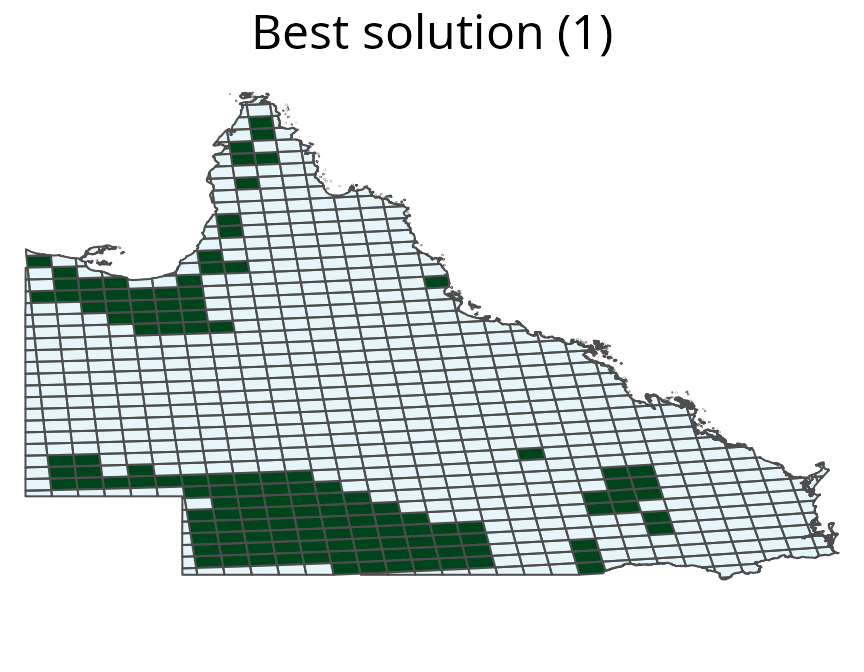
\includegraphics[width=3.5in,height=3.5in]{rapr_files/figure-latex/unnamed-chunk-58-1} 

}

\caption{A multi-species prioritisation for the uniformly, normally, and bimodally distributed species generated using only amount-based targets (20\%). Additionally, this priorititisation was specified to have high connectivity, by using a high $BLM$ parameter. See Figure 12 caption for conventions.}\label{fig:unnamed-chunk-58}
\end{figure}

\begin{Shaded}
\begin{Highlighting}[]
\CommentTok{# difference between the two prioritisations}
\KeywordTok{plot}\NormalTok{(sim_mrs_amount_blm, sim_mrs_amount, }\DecValTok{1}\NormalTok{, }\DecValTok{1}\NormalTok{, }\DataTypeTok{main=}\StringTok{'Difference between solutions'}\NormalTok{)}
\end{Highlighting}
\end{Shaded}

\begin{figure}

{\centering 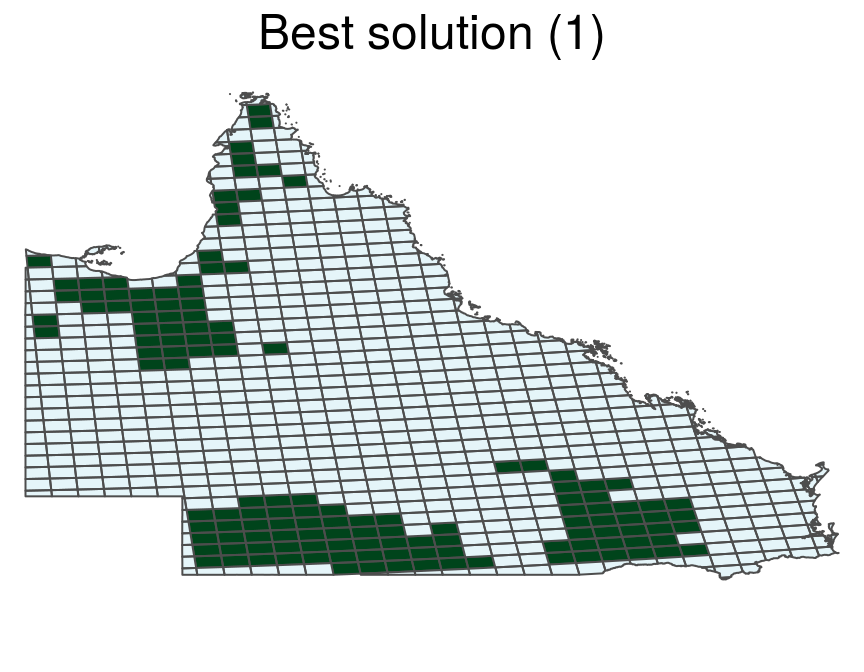
\includegraphics[width=3.5in,height=3.5in]{rapr_files/figure-latex/unnamed-chunk-59-1} 

}

\caption{Difference between two multi-species prioritisations. See Figure 7 caption for conventions.}\label{fig:unnamed-chunk-59}
\end{figure}

Here we can see that the prioritisation generated using a \texttt{BLM}
parameter of 100 is much more clustered than the prioritisation
generated using a \texttt{BLM} of 0. In practice, conservation planners
will need to try a variety of \texttt{BLM} parameters to find a suitable
prioritisation.

\subsubsection{Complex simulated
species}\label{complex-simulated-species}

\paragraph{Data}\label{data-1}

In the previous examples, we have only used Euclidean distances to
determine how much of an attribute space is sampled by a prioritisation.
However, Euclidean distances can be poor measures of distance for
multivariate, binary, or correlated variables (Faith \emph{et al.}
1987). As a consequence this may lead to over- or under-estimates of the
quality of a given solution.

The \texttt{rapr} R package provides a suite of distance metrics that
can be used to calculate spatial representation (see
\texttt{?AttributeSpace} for available metrics and their equations). To
illustrate how using different distance metrics can affect the optimal
solution, we will generate a new suite of prioritisations using
different distance metrics.

First, we will simulate a new species and a three-dimensional attribute
space. Note that unlike the previous examples, the attribute space will
not be geographic space. Rather, each dimension in the attribute space
will have values that map onto geographic space (eg. like climatic
variables across the landscape). To add further complexity, we simulate
their distributions using Gaussian processes.

\begin{Shaded}
\begin{Highlighting}[]
\CommentTok{# set seed for simulations}
\KeywordTok{set.seed}\NormalTok{(}\DecValTok{500}\NormalTok{)}

\NormalTok{## simulate planning units}
\NormalTok{sim_pus <-}\StringTok{ }\KeywordTok{sim.pus}\NormalTok{(25L)}

\CommentTok{# simulate species}
\NormalTok{sim_gspp <-}\StringTok{ }\KeywordTok{sim.species}\NormalTok{(sim_pus, }\DataTypeTok{model=}\KeywordTok{RPgauss}\NormalTok{(), }\DataTypeTok{n=}\DecValTok{1}\NormalTok{, }\DataTypeTok{res=}\FloatTok{0.1}\NormalTok{)}

\CommentTok{# simulate space}
\NormalTok{sim_gspace <-}\StringTok{ }\KeywordTok{sim.space}\NormalTok{(sim_pus, }\DataTypeTok{model=}\KeywordTok{RMgauss}\NormalTok{(}\DataTypeTok{scale=}\DecValTok{3}\NormalTok{), }\DataTypeTok{d=}\DecValTok{3}\NormalTok{, }\DataTypeTok{res=}\FloatTok{0.1}\NormalTok{)}
\end{Highlighting}
\end{Shaded}

\begin{verbatim}
## ...
\end{verbatim}

\begin{Shaded}
\begin{Highlighting}[]
\CommentTok{# increment simulated space values by 100 so there are no negative values}
\CommentTok{# so we can investigate all distance metrics}
\NormalTok{sim_gspace <-}\StringTok{ }\NormalTok{sim_gspace +}\StringTok{ }\DecValTok{100}
\end{Highlighting}
\end{Shaded}

\begin{Shaded}
\begin{Highlighting}[]
\CommentTok{# generate RapUnsolved object containing data to generate prioritisations}
\NormalTok{sim_ru_gp <-}\StringTok{ }\KeywordTok{rap}\NormalTok{(}
    \NormalTok{sim_pus, sim_gspp, sim_gspace, }
    \DataTypeTok{amount.target=}\FloatTok{0.2}\NormalTok{, }\DataTypeTok{space.target=}\FloatTok{0.85}\NormalTok{,}
    \DataTypeTok{n.demand.points=}\NormalTok{50L, }\DataTypeTok{kernel.method=}\StringTok{'hypervolume'}\NormalTok{,}
    \DataTypeTok{include.geographic.space=}\OtherTok{FALSE}\NormalTok{, }\DataTypeTok{scale=}\OtherTok{FALSE}\NormalTok{, }\DataTypeTok{solve=}\OtherTok{FALSE}
\NormalTok{)}
\end{Highlighting}
\end{Shaded}

\begin{verbatim}
## Choosing repsperpoint=1500 (use a larger value for more accuracy.)
## Evaluating probability density...
## Building tree... done.
## Querying tree... 2.33918e-06  0.0233942  0.046786  0.0701778  0.0935696  0.116961  0.140353  0.163745  0.187137  0.210529  0.23392  0.257312  0.280704  0.304096  0.327488  0.35088  0.374271  0.397663  0.421055  0.444447  0.467839  0.49123  0.514622  0.538014  0.561406  0.584798  0.608189  0.631581  0.654973  0.678365  0.701757  0.725149  0.74854  0.771932  0.795324  0.818716  0.842108  0.865499  0.888891  0.912283  0.935675  0.959067  0.982458  done.
## Finished evaluating probability density.
## Beginning volume calculation... done. 
## Quantile requested: 0.20   obtained: 0.20
\end{verbatim}

Let's visualise the species' distribution and the distribution of the
attribute space across geographic space.

\begin{Shaded}
\begin{Highlighting}[]
\CommentTok{# plot species distribution}
\KeywordTok{plot}\NormalTok{(}
    \NormalTok{sim_gspp,}
    \DataTypeTok{main=}\StringTok{'Simulated species'}\NormalTok{,}
    \DataTypeTok{col=}\KeywordTok{colorRampPalette}\NormalTok{(}\KeywordTok{c}\NormalTok{(}\StringTok{"#FFFFD9"}\NormalTok{, }\StringTok{"#EDF8B1"}\NormalTok{, }\StringTok{"#C7E9B4"}\NormalTok{, }\StringTok{"#7FCDBB"}\NormalTok{,}
        \StringTok{"#41B6C4"}\NormalTok{, }\StringTok{"#1D91C0"}\NormalTok{, }\StringTok{"#225EA8"}\NormalTok{, }\StringTok{"#253494"}\NormalTok{, }\StringTok{"#081D58"}
    \NormalTok{))(}\DecValTok{100}\NormalTok{)}
\NormalTok{)}
\KeywordTok{lines}\NormalTok{(sim_pus)}
\end{Highlighting}
\end{Shaded}

\begin{figure}

{\centering 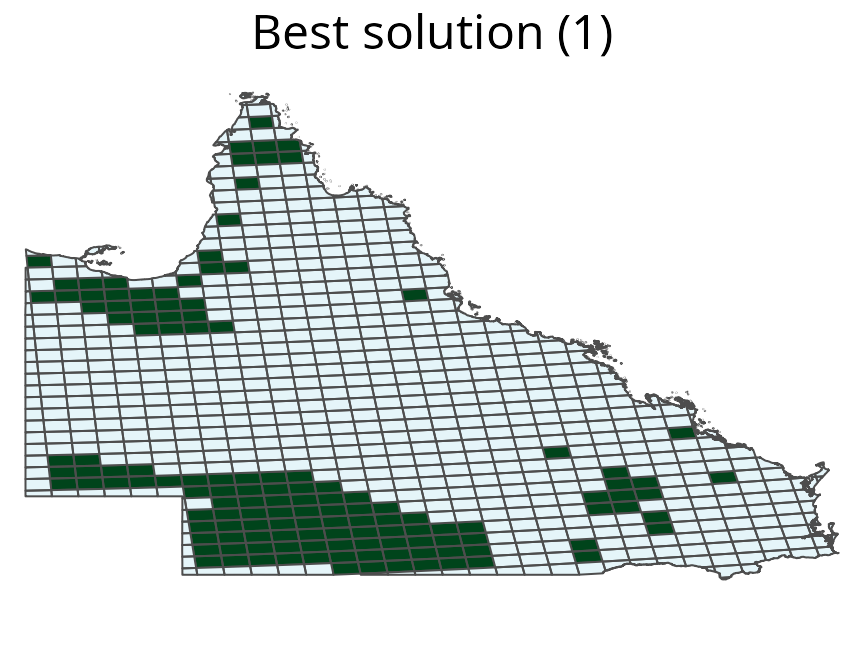
\includegraphics[width=3.5in,height=3.5in]{rapr_files/figure-latex/unnamed-chunk-62-1} 

}

\caption{Distribution map of a species simulated using Gaussian prorceses. See Figure 2 caption for conventions.}\label{fig:unnamed-chunk-62}
\end{figure}

\begin{Shaded}
\begin{Highlighting}[]
\CommentTok{# plot distribution of each dimension in the attribute space across geographic space}
\KeywordTok{plot}\NormalTok{(}
    \NormalTok{sim_gspace,}
    \DataTypeTok{main=}\KeywordTok{c}\NormalTok{(}\StringTok{'Attribute space (d=1)'}\NormalTok{, }\StringTok{'Attribute space (d=2)'}\NormalTok{, }\StringTok{'Attribute space (d=3)'}\NormalTok{),}
    \DataTypeTok{addfun=}\NormalTok{function()\{}\KeywordTok{lines}\NormalTok{(sim_pus)\},}
    \DataTypeTok{nc=}\DecValTok{3}
\NormalTok{)}
\end{Highlighting}
\end{Shaded}

\begin{figure}

{\centering 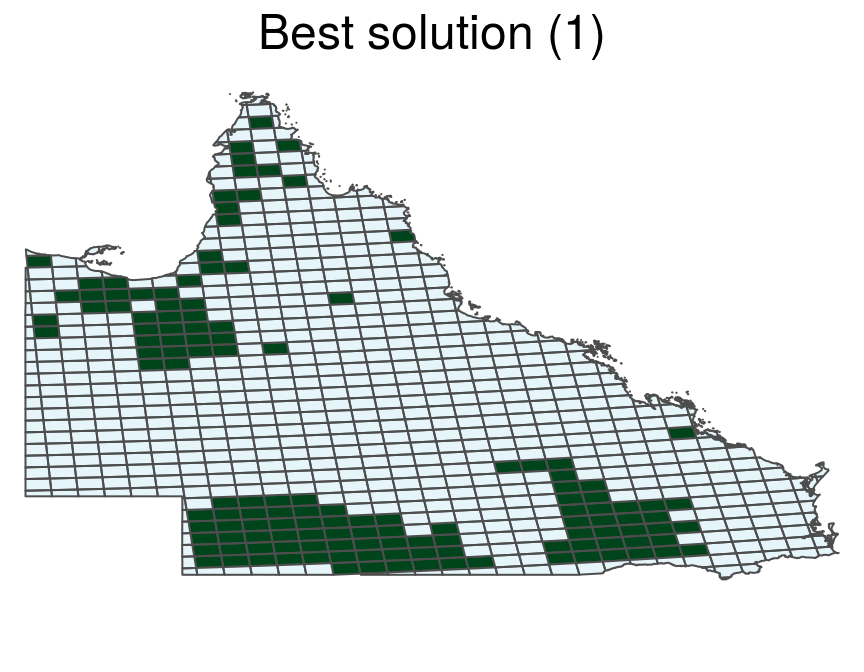
\includegraphics[width=7in,height=2.5in]{rapr_files/figure-latex/unnamed-chunk-63-1} 

}

\caption{Distribution of spatial variables across the species' geographic range. These variables each represent a dimension of a three-dimensional attribute space.}\label{fig:unnamed-chunk-63}
\end{figure}

\paragraph{Distance metrics}\label{distance-metrics}

For each different distance metric, we will update the \texttt{sim\_gru}
object with the new distance metric, solve it, and store the solution in
a list.

\begin{Shaded}
\begin{Highlighting}[]
\CommentTok{# create vector with distance metrics}
\NormalTok{dist.metrics <-}\StringTok{ }\KeywordTok{c}\NormalTok{(}
    \StringTok{'euclidean'}\NormalTok{, }\StringTok{'bray'}\NormalTok{, }\StringTok{'manhattan'}\NormalTok{,}\StringTok{'gower'}\NormalTok{,}
    \StringTok{'canberra'}\NormalTok{, }\StringTok{'mahalanobis'}\NormalTok{,}
    \StringTok{'jaccard'}\NormalTok{, }\StringTok{'kulczynski'}
\NormalTok{)}

\CommentTok{# generate solutions}
\NormalTok{solutions <-}\StringTok{ }\KeywordTok{list}\NormalTok{()}
\NormalTok{for (i in dist.metrics) \{}
    \NormalTok{solutions[[i]] <-}\StringTok{ }\KeywordTok{update}\NormalTok{(sim_ru_gp, }\DataTypeTok{distance.metric=}\NormalTok{i)}
\NormalTok{\}}
\end{Highlighting}
\end{Shaded}

Now, let's plot the solutions to see how they differ.

\begin{Shaded}
\begin{Highlighting}[]
\CommentTok{# set plotting window}
\KeywordTok{par}\NormalTok{(}\DataTypeTok{mfrow=}\KeywordTok{c}\NormalTok{(}\DecValTok{3}\NormalTok{,}\DecValTok{3}\NormalTok{), }\DataTypeTok{mar=}\KeywordTok{c}\NormalTok{(}\DecValTok{0}\NormalTok{, }\DecValTok{0}\NormalTok{, }\FloatTok{4.1}\NormalTok{, }\DecValTok{0}\NormalTok{))}

\NormalTok{## create plots showing the selected planning units (dark green)}
\NormalTok{for (i in }\KeywordTok{seq_along}\NormalTok{(solutions)) \{}
    \CommentTok{# plot i'th solution}
    \KeywordTok{plot}\NormalTok{(}
        \NormalTok{sim_pus,}
        \DataTypeTok{main=}\NormalTok{dist.metrics[i],}
        \DataTypeTok{col=}\KeywordTok{replace}\NormalTok{(}
            \KeywordTok{rep}\NormalTok{(}\StringTok{'#ccece6'}\NormalTok{,}\KeywordTok{nrow}\NormalTok{(sim_pus@data)),}
            \KeywordTok{which}\NormalTok{(}\KeywordTok{selections}\NormalTok{(solutions[[i]])==}\DecValTok{1}\NormalTok{),}
            \StringTok{'#00441b'}
        \NormalTok{),}
        \DataTypeTok{axes=}\OtherTok{FALSE}
    \NormalTok{)}
\NormalTok{\}}

\CommentTok{# reset plotting window}
\KeywordTok{par}\NormalTok{(}\DataTypeTok{mfrow=}\KeywordTok{c}\NormalTok{(}\DecValTok{1}\NormalTok{,}\DecValTok{1}\NormalTok{), }\DataTypeTok{mar=}\KeywordTok{c}\NormalTok{(}\FloatTok{5.1}\NormalTok{, }\FloatTok{4.1}\NormalTok{, }\FloatTok{4.1}\NormalTok{, }\FloatTok{2.1}\NormalTok{))}
\end{Highlighting}
\end{Shaded}

\begin{figure}[htbp]
\centering
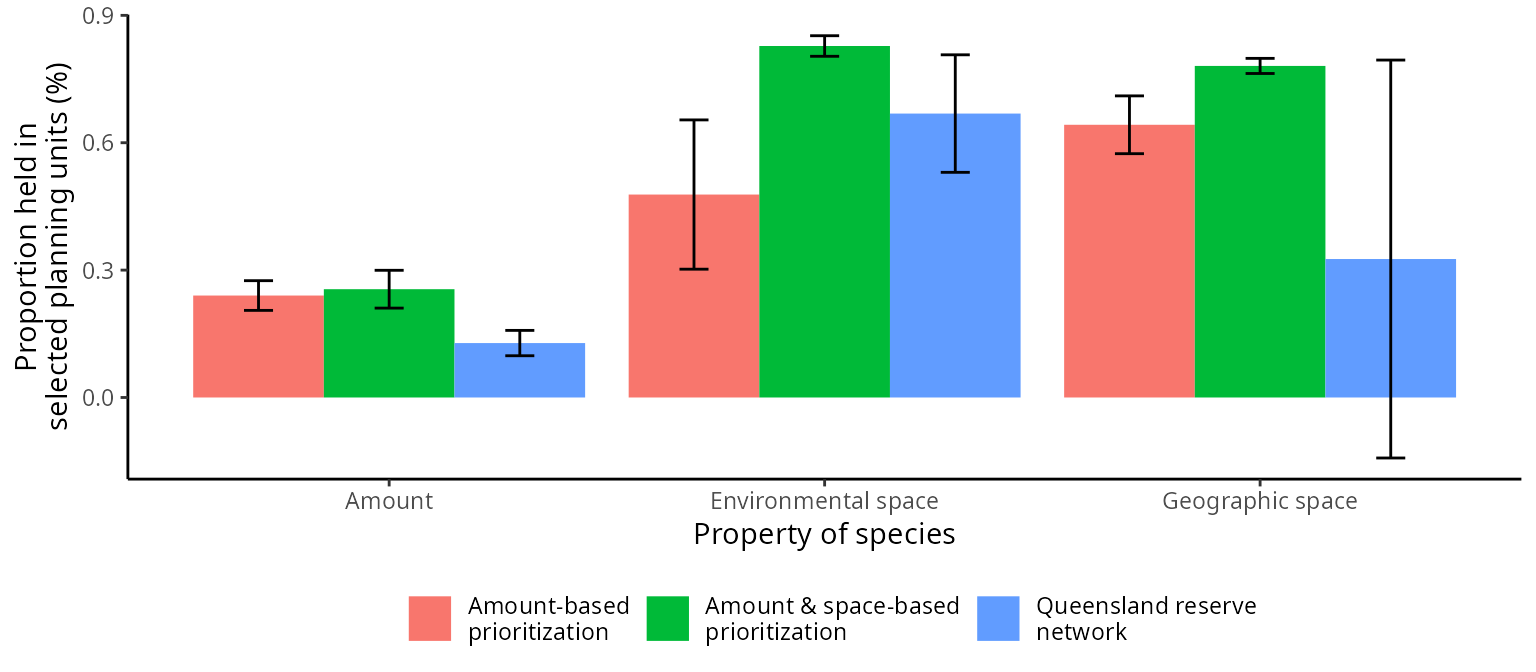
\includegraphics{rapr_files/figure-latex/unnamed-chunk-66-1.pdf}
\caption{Prioritisations generated using different distance metrics. See
Figure 12 for conventions.}
\end{figure}

It appears that main difference between the solutions is which planning
units get selected in the bottom section of the study area. Some
solutions tend to select a lot of planning units in this region (eg.
Euclidean, Gower, and Manhattan), whereas others select fewer planning
units (eg. Bray-Curtis, Jaccard, and Kulczynski). Conservation planners
should think carefully which distance metric is most appropriate for
their attribute spaces. See the discussion section below for guidelines
on selecting an appropriate distance metric.

\subsubsection{Case-study examples}\label{case-study-examples}

\paragraph{Overview}\label{overview}

Here we will investigate how space-based targets can affect
prioritisations using a more realistic dataset. We will generate
prioritisations for the four bird species--
\href{http://www.birdlife.org/datazone/speciesfactsheet.php?id=1092\&gclid=CjwKEAiApYGyBRC-g_jIstuduV8SJABCEzhZoONUy8VlwRZqeFB1Z5M03CjyneIvX8KdVKIPZvckrRoCgJDw_wcB}{blue-winged
kookaburra},
\href{http://www.birdlife.org/datazone/species/factsheet/22704394?gclid=CjwKEAiApYGyBRC-g_jIstuduV8SJABCEzhZHxCTcR38YnFlhePYt19gD31lqxxwrMmtIuWFhUwLmRoCGJjw_wcB}{brown-backed
honeyeater},
\href{http://www.birdlife.org/datazone/speciesfactsheet.php?id=3588}{brown
falcon},
\href{http://www.birdlife.org/datazone/speciesfactsheet.php?id=1466}{pale-headed
rosella}--in Queensland, Australia. This region contains a broad range
of different habitats--such as rainforests, woodlands, and
deserts--making it ideal for this tutorial. First, we will generate a
typical amount-based prioritisation that aims to capture 20\% of the
species' distributions. Then we will generate a prioritisation that also
aims to secure populations in representative parts of the species'
distributions in terms of their geographic location and their
environmental heterogeneity. To do this we will generate a
prioritisation using 20\% amount-based targets and 85\% space-based
targets. Finally, we will compare these prioritisations to Australia's
existing protected network.

\paragraph{Data}\label{data-2}

Survey data for the species were obtained from
\href{http://birdlife.org.au/projects/atlas-and-birdata}{BirdLife
Australia}. The survey data was rarefied using a 100km$^2$ grid, wherein
the survey with the greatest number of repeat visits in each grid cell
was chosen. To model the distribution of each species, environmental
data were obtained at survey location (site). Specifically,
\href{http://www.worldclim.org/bioclim}{climatic data} (bio1, bio4,
bio15, bio16, bio17) and
\href{http://www.environment.gov.au/fed/catalog/search/resource/details.page?uuid=\%7BEBBCC6FA-8C13-422A-BCD7-24A9F8B52A9A\%7D}{classifications
of the vegetation at the site} were used. Occupancy-detection models
(MacKenzie \emph{et al.} 2002) were fit using Stan (Stan Development
Team 2015) using manually tuned parameters (adapt deta=0.9, maximum
treedepth=20, chains=4 , warmup iterations=1000, total iterations=1500)
with five-fold cross-validation. In each replicate, data were
partitioned into training and test sites. A full model was fit using
quadratic terms for environmental variables in the site-component, and
an intercept in the detection-component of the model. The full model was
then subject to a step-wise backwards term deletion routine. Terms were
retained when their inclusion resulted in a model with a greater area
under the curve (AUC) value as calculated using the test data. Maps were
generated for each species as an average of the predictions from the
best model in each best replicate. To further improve the accuracy of
these maps, areas well outside of the species' known distributions were
set to 0. For each species, this was achieved by masking out
\href{https://www.environment.gov.au/land/nrs/science/ibra}{biogeographic
regions} where the species was not observed, and regions that did not
have a neighbouring planning unit where the species was observed. The
maps were then resampled (10km$^2$ resolution) and cropped to the study
area. The resulting maps are stored in the \texttt{cs\_spp} object.

\begin{Shaded}
\begin{Highlighting}[]
\CommentTok{# load data}
\KeywordTok{data}\NormalTok{(cs_spp)}

\CommentTok{# plot species' distributions}
\KeywordTok{plot}\NormalTok{(cs_spp, }\DataTypeTok{main=}\KeywordTok{c}\NormalTok{(}
    \StringTok{"Blue-winged kookaburra"}\NormalTok{, }\StringTok{"Brown-backed honeyeater"}\NormalTok{, }
    \StringTok{"Brown falcon"}\NormalTok{, }\StringTok{"Pale-headed rosella"}
\NormalTok{))}
\end{Highlighting}
\end{Shaded}

\begin{figure}[htbp]
\centering
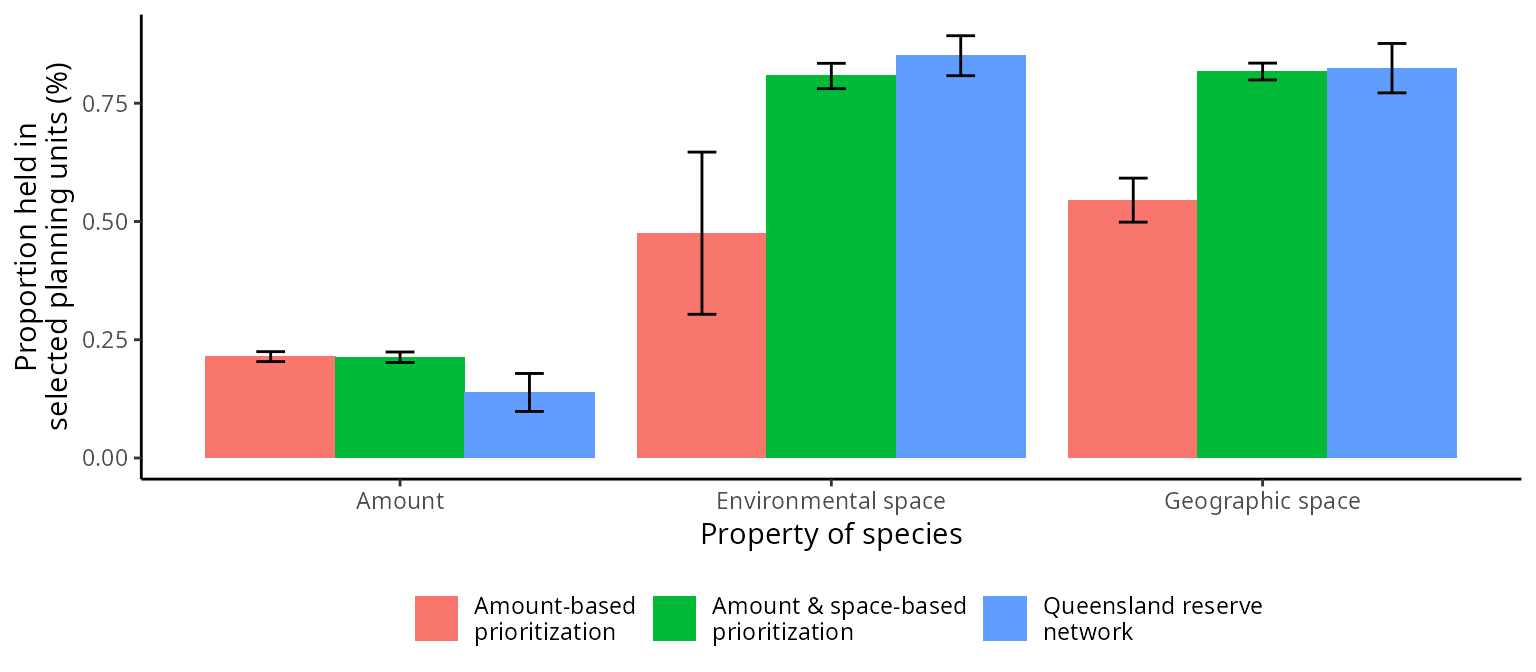
\includegraphics{rapr_files/figure-latex/unnamed-chunk-67-1.pdf}
\caption{Distribution map for four Australian bird species. Pixel
colours denote probability of occupancy.}
\end{figure}

Planning units (50km$^2$ resolution) were generated across Australia,
and then clipped to the
\href{http://www.abs.gov.au/ausstats/abs@.nsf/mf/1259.0.30.001?OpenDocument}{Queensland
state borders and coastline}. \textbf{Note that we are using excessively
coarse planning units so that our examples will complete relatively
quickly. In a real-world planning exercise, we would use much finer
planning units.} To compare our prioritisations to
\href{http://www.protectedplanet.net/country/AU}{Queensland's existing
protected area network}, this network was intersected with the planning
units. Planning units with more than 50\% of their area inside a
protected area had their status set to 2
(\href{http://www.uq.edu.au/marxan/tutorial/module4.html}{following
conventions in Marxan}). Since we do not have cost data, the
prioritisations will aim to select the minimum number of planning units
required to meet the targets. The planning units are stored in the
\texttt{cs\_pu} object.

\begin{Shaded}
\begin{Highlighting}[]
\CommentTok{# load data}
\KeywordTok{data}\NormalTok{(cs_pus)}

\NormalTok{## plot planning units}
\CommentTok{# convert SpatialPolygons to PolySet for quick plotting}
\NormalTok{cs_pus2 <-}\StringTok{ }\KeywordTok{SpatialPolygons2PolySet}\NormalTok{(cs_pus)}

\CommentTok{# create vector of colours for planning units}
\CommentTok{# + light green: units not already inside reserve}
\CommentTok{# + yellow: units already inside reserve}
\NormalTok{cs_pus_cols <-}\StringTok{ }\KeywordTok{rep}\NormalTok{(}\StringTok{'#c7e9c0'}\NormalTok{, }\KeywordTok{nrow}\NormalTok{(cs_pus@data))}
\NormalTok{cs_pus_cols[}\KeywordTok{which}\NormalTok{(cs_pus$status==}\DecValTok{2}\NormalTok{)] <-}\StringTok{ 'yellow'}

\CommentTok{# set plotting window}
\KeywordTok{par}\NormalTok{(}\DataTypeTok{mar=}\KeywordTok{c}\NormalTok{(}\FloatTok{0.1}\NormalTok{, }\FloatTok{0.1}\NormalTok{, }\FloatTok{4.1}\NormalTok{, }\FloatTok{0.1}\NormalTok{))}

\CommentTok{# plot polygons}
\NormalTok{PBSmapping::}\KeywordTok{plotPolys}\NormalTok{(}
    \NormalTok{cs_pus2, }\DataTypeTok{col=}\NormalTok{cs_pus_cols, }\DataTypeTok{border=}\StringTok{'gray30'}\NormalTok{, }
    \DataTypeTok{xlab=}\StringTok{''}\NormalTok{, }\DataTypeTok{ylab=}\StringTok{''}\NormalTok{, }\DataTypeTok{axes=}\OtherTok{FALSE}\NormalTok{, }
    \DataTypeTok{main=}\StringTok{'Case-study planning units'}
\NormalTok{)}
\end{Highlighting}
\end{Shaded}

\begin{figure}

{\centering \includegraphics[width=3.5in,height=3.5in]{rapr_files/figure-latex/unnamed-chunk-68-1} 

}

\caption{Planning units for the case-study examples. Yellow polygons represent planning units with more then 50\% of their area already in existing reserves.}\label{fig:unnamed-chunk-68}
\end{figure}

\begin{Shaded}
\begin{Highlighting}[]
\CommentTok{# reset plotting window}
\KeywordTok{par}\NormalTok{(}\DataTypeTok{mar=}\KeywordTok{c}\NormalTok{(}\FloatTok{5.1}\NormalTok{, }\FloatTok{4.1}\NormalTok{, }\FloatTok{4.1}\NormalTok{, }\FloatTok{2.1}\NormalTok{))}
\end{Highlighting}
\end{Shaded}

To map the distribution of environmental conditions across the species'
range, 21 \href{http://www.worldclim.org/bioclim}{bioclimatic layers}
were obtained. These layers were cropped to Australia and subject to
\href{http://cc.oulu.fi/~jarioksa/softhelp/vegan/html/decorana.html}{detrended
correspondence analysis} to produce two new variables. These layers are
stored in the \texttt{cs\_space} object.

\begin{Shaded}
\begin{Highlighting}[]
\CommentTok{# load data}
\KeywordTok{data}\NormalTok{(cs_space)}

\CommentTok{# plot variables}
\KeywordTok{plot}\NormalTok{(cs_space, }\DataTypeTok{main=}\KeywordTok{c}\NormalTok{(}\StringTok{'DC1'}\NormalTok{, }\StringTok{'DC2'}\NormalTok{))}
\end{Highlighting}
\end{Shaded}

\begin{figure}[htbp]
\centering
\includegraphics{rapr_files/figure-latex/unnamed-chunk-69-1.pdf}
\caption{Broad-scale environmental variation across Australia. The
variable DC1 describes the transition from wet and cool to dry and hot
conditions. The variable DC2 describes the transition from wet and hot
to dry and cool conditions.}
\end{figure}

\paragraph{Effectiveness of Australia's reserve network compared to
optimal
prioritisations}\label{effectiveness-of-australias-reserve-network-compared-to-optimal-prioritisations}

To simplify the process of formatting data and generating
prioritisations, we can use the \texttt{rap} function. First, we will
generate an amount-based prioritisation that aims to capture 20\% of the
rosella's range. We will use 50 demand points to map the geographic and
environmental spaces. \textbf{Be warned, the examples hereafter can take
5-10 minutes to run.}

\begin{Shaded}
\begin{Highlighting}[]
\CommentTok{# make amount-based prioritisation,}
\CommentTok{# and ignore existing protected areas by discarding values in the }
\CommentTok{# status (third) column of the attribute table}
\NormalTok{cs_rs_amount <-}\StringTok{ }\KeywordTok{rap}\NormalTok{(}
    \NormalTok{cs_pus[,-}\DecValTok{2}\NormalTok{], cs_spp, cs_space,}
  \DataTypeTok{amount.target=}\FloatTok{0.2}\NormalTok{, }\DataTypeTok{space.target=}\OtherTok{NA}\NormalTok{, }\DataTypeTok{n.demand.points=}\NormalTok{50L,}
  \DataTypeTok{include.geographic.space=}\OtherTok{TRUE}\NormalTok{, }\DataTypeTok{formulation=}\StringTok{'unreliable'}\NormalTok{,}
  \DataTypeTok{solve=}\OtherTok{FALSE}
\NormalTok{)}
\end{Highlighting}
\end{Shaded}

\begin{verbatim}
## Warning in (function (pus, species, spaces = NULL, amount.target = 0.2, :
## argument to pus does not have a 'status' column, creating default with all
## status=0L
\end{verbatim}

\begin{Shaded}
\begin{Highlighting}[]
\CommentTok{# threshold probabilities to 0.1 for space calculations}
\NormalTok{cs_rs_amount <-}\StringTok{ }\KeywordTok{prob.subset}\NormalTok{(cs_rs_amount, }\DataTypeTok{species=}\DecValTok{1}\NormalTok{:}\DecValTok{4}\NormalTok{, }\DataTypeTok{threshold=}\KeywordTok{rep}\NormalTok{(}\FloatTok{0.1}\NormalTok{,}\DecValTok{4}\NormalTok{))}
\end{Highlighting}
\end{Shaded}

\begin{Shaded}
\begin{Highlighting}[]
\CommentTok{# generate prioritisation}
\NormalTok{cs_rs_amount <-}\StringTok{ }\KeywordTok{solve}\NormalTok{(cs_rs_amount)}
\end{Highlighting}
\end{Shaded}

\begin{Shaded}
\begin{Highlighting}[]
\CommentTok{# show summary}
\KeywordTok{summary}\NormalTok{(cs_rs_amount)}
\end{Highlighting}
\end{Shaded}

\begin{verbatim}
##   Run_Number Status Score Cost Planning_Units Connectivity_Total
## 1          1 MANUAL   136  136            136           98882414
##   Connectivity_In Connectivity_Edge Connectivity_Out
## 1         9636021          81120163          8126230
##   Connectivity_In_Fraction
## 1               0.09744929
\end{verbatim}

\begin{Shaded}
\begin{Highlighting}[]
\CommentTok{# plot prioritisation}
\KeywordTok{plot}\NormalTok{(cs_rs_amount, }\DecValTok{1}\NormalTok{)}
\end{Highlighting}
\end{Shaded}

\begin{figure}

{\centering \includegraphics[width=3.5in,height=3.5in]{rapr_files/figure-latex/unnamed-chunk-73-1} 

}

\caption{Multi-species prioritisation generated for four bird species using amount-based targets (20\%). See Figure 12 captions for conventions.}\label{fig:unnamed-chunk-73}
\end{figure}

We can also see how well the prioritisation secures the species'
distributions in the geographic and environmental attribute spaces.

\begin{Shaded}
\begin{Highlighting}[]
\CommentTok{# plot prioritisation in geographic attribute space}
\NormalTok{p1 <-}\StringTok{ }\KeywordTok{space.plot}\NormalTok{(cs_rs_amount, }\DecValTok{1}\NormalTok{, }\DecValTok{2}\NormalTok{, }\DataTypeTok{main=}\StringTok{'Blue-winged kookaburra'}\NormalTok{)}
\NormalTok{p2 <-}\StringTok{ }\KeywordTok{space.plot}\NormalTok{(cs_rs_amount, }\DecValTok{2}\NormalTok{, }\DecValTok{2}\NormalTok{, }\DataTypeTok{main=}\StringTok{'Brown-backed honeyeater'}\NormalTok{)}
\NormalTok{p3 <-}\StringTok{ }\KeywordTok{space.plot}\NormalTok{(cs_rs_amount, }\DecValTok{3}\NormalTok{, }\DecValTok{2}\NormalTok{, }\DataTypeTok{main=}\StringTok{'Brown falcon'}\NormalTok{)}
\NormalTok{p4 <-}\StringTok{ }\KeywordTok{space.plot}\NormalTok{(cs_rs_amount, }\DecValTok{4}\NormalTok{, }\DecValTok{2}\NormalTok{, }\DataTypeTok{main=}\StringTok{'Pale-headed rosella'}\NormalTok{)}
\NormalTok{gridExtra::}\KeywordTok{grid.arrange}\NormalTok{(p1, p2, p3, p4, }\DataTypeTok{ncol=}\DecValTok{2}\NormalTok{)}
\end{Highlighting}
\end{Shaded}

\begin{figure}[htbp]
\centering
\includegraphics{rapr_files/figure-latex/unnamed-chunk-74-1.pdf}
\caption{Distribution of amount-based prioritisation in the geographic
attribute space. Points denote combinations of environmental conditions.
Green and grey points represent planning unit selected for and not
selected for prioritisation (respectively). Blue points denote demand
points, and their size indicates their weighting.}
\end{figure}

\begin{Shaded}
\begin{Highlighting}[]
\CommentTok{# plot prioritisation in environmental attribute space}
\NormalTok{p1 <-}\StringTok{ }\KeywordTok{space.plot}\NormalTok{(cs_rs_amount, }\DecValTok{1}\NormalTok{, }\DecValTok{1}\NormalTok{, }\DataTypeTok{main=}\StringTok{'Blue-winged kookaburra'}\NormalTok{)}
\NormalTok{p2 <-}\StringTok{ }\KeywordTok{space.plot}\NormalTok{(cs_rs_amount, }\DecValTok{2}\NormalTok{, }\DecValTok{1}\NormalTok{, }\DataTypeTok{main=}\StringTok{'Brown-backed honeyeater'}\NormalTok{)}
\NormalTok{p3 <-}\StringTok{ }\KeywordTok{space.plot}\NormalTok{(cs_rs_amount, }\DecValTok{3}\NormalTok{, }\DecValTok{1}\NormalTok{, }\DataTypeTok{main=}\StringTok{'Brown falcon'}\NormalTok{)}
\NormalTok{p4 <-}\StringTok{ }\KeywordTok{space.plot}\NormalTok{(cs_rs_amount, }\DecValTok{4}\NormalTok{, }\DecValTok{1}\NormalTok{, }\DataTypeTok{main=}\StringTok{'Pale-headed rosella'}\NormalTok{)}
\NormalTok{gridExtra::}\KeywordTok{grid.arrange}\NormalTok{(p1, p2, p3, p4, }\DataTypeTok{ncol=}\DecValTok{2}\NormalTok{)}
\end{Highlighting}
\end{Shaded}

\begin{figure}[htbp]
\centering
\includegraphics{rapr_files/figure-latex/unnamed-chunk-75-1.pdf}
\caption{Distribution of amount-based prioritisation in the
environmental attribute space. See Figure 28 caption for conventions.}
\end{figure}

Next, let's generate a prioritisation using amount- and space-based
targets. This prioritisation will secure 50\% of the species
distribution in geographic and environmental space.

\begin{Shaded}
\begin{Highlighting}[]
\CommentTok{# make amount- and space-based prioritisation}
\NormalTok{cs_rs_space <-}\StringTok{ }\KeywordTok{update}\NormalTok{(cs_rs_amount, }\DataTypeTok{space.target=}\FloatTok{0.5}\NormalTok{)}
\end{Highlighting}
\end{Shaded}

\begin{Shaded}
\begin{Highlighting}[]
\CommentTok{# show summary}
\KeywordTok{summary}\NormalTok{(cs_rs_space)}
\end{Highlighting}
\end{Shaded}

\begin{verbatim}
##   Run_Number Status Score Cost Planning_Units Connectivity_Total
## 1          1 MANUAL   137  137            137           98882414
##   Connectivity_In Connectivity_Edge Connectivity_Out
## 1         9738090          80918598          8225726
##   Connectivity_In_Fraction
## 1               0.09848151
\end{verbatim}

\begin{Shaded}
\begin{Highlighting}[]
\CommentTok{# plot prioritisation}
\KeywordTok{plot}\NormalTok{(cs_rs_space,}\DecValTok{1}\NormalTok{)}
\end{Highlighting}
\end{Shaded}

\begin{center}\includegraphics[width=3.5in,height=3.5in]{rapr_files/figure-latex/unnamed-chunk-78-1} \end{center}

\begin{Shaded}
\begin{Highlighting}[]
\CommentTok{# plot prioritisation in geographic attribute space}
\NormalTok{p1 <-}\StringTok{ }\KeywordTok{space.plot}\NormalTok{(cs_rs_space, }\DecValTok{1}\NormalTok{, }\DecValTok{2}\NormalTok{, }\DataTypeTok{main=}\StringTok{'Blue-winged kookaburra'}\NormalTok{)}
\NormalTok{p2 <-}\StringTok{ }\KeywordTok{space.plot}\NormalTok{(cs_rs_space, }\DecValTok{2}\NormalTok{, }\DecValTok{2}\NormalTok{, }\DataTypeTok{main=}\StringTok{'Brown-backed honeyeater'}\NormalTok{)}
\NormalTok{p3 <-}\StringTok{ }\KeywordTok{space.plot}\NormalTok{(cs_rs_space, }\DecValTok{3}\NormalTok{, }\DecValTok{2}\NormalTok{, }\DataTypeTok{main=}\StringTok{'Brown falcon'}\NormalTok{)}
\NormalTok{p4 <-}\StringTok{ }\KeywordTok{space.plot}\NormalTok{(cs_rs_space, }\DecValTok{4}\NormalTok{, }\DecValTok{2}\NormalTok{, }\DataTypeTok{main=}\StringTok{'Pale-headed rosella'}\NormalTok{)}
\NormalTok{gridExtra::}\KeywordTok{grid.arrange}\NormalTok{(p1, p2, p3, p4, }\DataTypeTok{ncol=}\DecValTok{2}\NormalTok{)}
\end{Highlighting}
\end{Shaded}

\begin{figure}[htbp]
\centering
\includegraphics{rapr_files/figure-latex/unnamed-chunk-79-1.pdf}
\caption{Distribution of the amount- and space-based prioritisation in
the geographic attribute space. See Figure 28 caption for conventions.}
\end{figure}

\begin{Shaded}
\begin{Highlighting}[]
\CommentTok{# plot prioritisation in environmental attribute space}
\NormalTok{p1 <-}\StringTok{ }\KeywordTok{space.plot}\NormalTok{(cs_rs_space, }\DecValTok{1}\NormalTok{, }\DecValTok{1}\NormalTok{, }\DataTypeTok{main=}\StringTok{'Blue-winged kookaburra'}\NormalTok{)}
\NormalTok{p2 <-}\StringTok{ }\KeywordTok{space.plot}\NormalTok{(cs_rs_space, }\DecValTok{2}\NormalTok{, }\DecValTok{1}\NormalTok{, }\DataTypeTok{main=}\StringTok{'Brown-backed honeyeater'}\NormalTok{)}
\NormalTok{p3 <-}\StringTok{ }\KeywordTok{space.plot}\NormalTok{(cs_rs_space, }\DecValTok{3}\NormalTok{, }\DecValTok{1}\NormalTok{, }\DataTypeTok{main=}\StringTok{'Brown falcon'}\NormalTok{)}
\NormalTok{p4 <-}\StringTok{ }\KeywordTok{space.plot}\NormalTok{(cs_rs_space, }\DecValTok{4}\NormalTok{, }\DecValTok{1}\NormalTok{, }\DataTypeTok{main=}\StringTok{'Pale-headed rosella'}\NormalTok{)}
\NormalTok{gridExtra::}\KeywordTok{grid.arrange}\NormalTok{(p1, p2, p3, p4, }\DataTypeTok{ncol=}\DecValTok{2}\NormalTok{)}
\end{Highlighting}
\end{Shaded}

\begin{figure}[htbp]
\centering
\includegraphics{rapr_files/figure-latex/unnamed-chunk-80-1.pdf}
\caption{Distribution of the amount- and space-based prioritisation in
the environmental attribute space. See Figure 28 caption for
conventions.}
\end{figure}

Let's compare these prioritisations with Queensland's existing protected
areas system. To do this, we can create update the
\texttt{cs\_rs\_space} with manually specified solutions to create a
\texttt{RapSolved} object to represent the Queensland's reserve network.

\begin{Shaded}
\begin{Highlighting}[]
\CommentTok{# generate vector with Australia's selections}
\NormalTok{aus_selections <-}\StringTok{ }\KeywordTok{which}\NormalTok{(cs_pus$status>}\DecValTok{0}\NormalTok{)}

\CommentTok{# create new object with Australia's network}
\NormalTok{cs_rs_aus <-}\StringTok{ }\KeywordTok{update}\NormalTok{(cs_rs_amount, }\DataTypeTok{b=}\NormalTok{aus_selections)}
\end{Highlighting}
\end{Shaded}

Now, let's plot the performance metrics for these prioritisations.

\begin{Shaded}
\begin{Highlighting}[]
\CommentTok{# define standard error function}
\NormalTok{se=function(x)\{}\KeywordTok{sd}\NormalTok{(x,}\DataTypeTok{na.rm=}\OtherTok{TRUE}\NormalTok{)/}\KeywordTok{sqrt}\NormalTok{(}\KeywordTok{sum}\NormalTok{(!}\KeywordTok{is.na}\NormalTok{(x)))\}}

\CommentTok{# create a table to store the values for the 3 prioritisations}
\NormalTok{cs_results <-}\StringTok{ }\KeywordTok{data.frame}\NormalTok{(}
    \DataTypeTok{name=}\KeywordTok{rep}\NormalTok{(}\KeywordTok{rep}\NormalTok{(}\KeywordTok{c}\NormalTok{(}\StringTok{'Amount-based prioritisation'}\NormalTok{, }
        \StringTok{'Amount+space-based prioritsation'}\NormalTok{, }\StringTok{'Queensland reserve network'}\NormalTok{),}
        \DataTypeTok{each=}\DecValTok{4}\NormalTok{),}\DecValTok{3}\NormalTok{),}
    \DataTypeTok{variable=}\KeywordTok{rep}\NormalTok{(}\KeywordTok{c}\NormalTok{(}\StringTok{'Amount'}\NormalTok{, }\StringTok{'Geographic space'}\NormalTok{, }\StringTok{'Environmental space'}\NormalTok{), }\DataTypeTok{each=}\DecValTok{12}\NormalTok{),}
    \DataTypeTok{species=}\KeywordTok{colnames}\NormalTok{(}\KeywordTok{amount.held}\NormalTok{(cs_rs_amount)),}
    \DataTypeTok{value=}\KeywordTok{c}\NormalTok{(}
        \KeywordTok{amount.held}\NormalTok{(cs_rs_amount)[}\DecValTok{1}\NormalTok{,], }\KeywordTok{amount.held}\NormalTok{(cs_rs_space)[}\DecValTok{1}\NormalTok{,],}
            \KeywordTok{amount.held}\NormalTok{(cs_rs_aus)[}\DecValTok{1}\NormalTok{,],}
        \KeywordTok{space.held}\NormalTok{(cs_rs_amount, }\DataTypeTok{space=}\DecValTok{2}\NormalTok{)[}\DecValTok{1}\NormalTok{,], }\KeywordTok{space.held}\NormalTok{(cs_rs_space, }\DataTypeTok{space=}\DecValTok{2}\NormalTok{)[}\DecValTok{1}\NormalTok{,], }
            \KeywordTok{space.held}\NormalTok{(cs_rs_aus, }\DataTypeTok{space=}\DecValTok{2}\NormalTok{)[}\DecValTok{1}\NormalTok{,],}
        \KeywordTok{space.held}\NormalTok{(cs_rs_amount, }\DataTypeTok{space=}\DecValTok{1}\NormalTok{)[}\DecValTok{1}\NormalTok{,], }\KeywordTok{space.held}\NormalTok{(cs_rs_space, }\DataTypeTok{space=}\DecValTok{1}\NormalTok{)[}\DecValTok{1}\NormalTok{,],}
            \KeywordTok{space.held}\NormalTok{(cs_rs_aus, }\DataTypeTok{space=}\DecValTok{1}\NormalTok{)[}\DecValTok{1}\NormalTok{,]}
    \NormalTok{)}
\NormalTok{) %>%}\StringTok{ }\KeywordTok{group_by}\NormalTok{(}
    \NormalTok{name,}
    \NormalTok{variable}
\NormalTok{) %>%}\StringTok{ }\KeywordTok{summarise}\NormalTok{(}
    \DataTypeTok{mean=}\KeywordTok{mean}\NormalTok{(value),}
    \DataTypeTok{se=}\KeywordTok{se}\NormalTok{(value)}
\NormalTok{)}

\CommentTok{# plot the performance metrics}
\KeywordTok{ggplot}\NormalTok{(}\KeywordTok{aes}\NormalTok{(}\DataTypeTok{x=}\NormalTok{variable, }\DataTypeTok{y=}\NormalTok{mean, }\DataTypeTok{fill=}\NormalTok{name), }\DataTypeTok{data=}\NormalTok{cs_results) +}
\StringTok{    }\KeywordTok{geom_bar}\NormalTok{(}\DataTypeTok{position=}\KeywordTok{position_dodge}\NormalTok{(}\FloatTok{0.9}\NormalTok{), }\DataTypeTok{stat=}\StringTok{'identity'}\NormalTok{) +}
\StringTok{    }\KeywordTok{geom_errorbar}\NormalTok{(}
        \KeywordTok{aes}\NormalTok{(}\DataTypeTok{ymin=}\NormalTok{mean-se, }\DataTypeTok{ymax=}\NormalTok{mean+se), }\DataTypeTok{position=}\KeywordTok{position_dodge}\NormalTok{(}\FloatTok{0.9}\NormalTok{),}
        \DataTypeTok{width=}\FloatTok{0.2}
    \NormalTok{) +}
\StringTok{    }\KeywordTok{xlab}\NormalTok{(}\StringTok{'Property of species'}\NormalTok{) +}
\StringTok{    }\KeywordTok{ylab}\NormalTok{(}\StringTok{'Proportion held in}\CharTok{\textbackslash{}n}\StringTok{selected planning units (%)'}\NormalTok{) +}
\StringTok{    }\KeywordTok{scale_fill_discrete}\NormalTok{(}
        \DataTypeTok{name=}\StringTok{''}
    \NormalTok{) +}
\StringTok{    }\KeywordTok{theme_classic}\NormalTok{() +}
\StringTok{    }\KeywordTok{theme}\NormalTok{(}\DataTypeTok{legend.position=}\StringTok{'bottom'}\NormalTok{,}\DataTypeTok{legend.direction=}\StringTok{'horizontal'}\NormalTok{)}
\end{Highlighting}
\end{Shaded}

\includegraphics{rapr_files/figure-latex/unnamed-chunk-82-1.pdf} We can
see that a greater number of planning units is needed to satisfy the
space-based targets. The prioritisation generated using just
amount-based targets has 136 planning units, and the prioritisations
using amount-based and space-based targets has 137 targets. These
results suggest that prioritisations based only on amount-based targets
can obtain a moderately representative sample of the species' geographic
distribution and climatic niche.

\subsection{Implications and future
directions}\label{implications-and-future-directions}

The \texttt{rapr} R package provides a unified approach to reserve
selection. This R package provides a decision maker with the tools to
generate prioritisations that secure an adequate amount of a
representative sample of biodiversity patterns and processes.
Additionally, the decision maker can accommodate uncertainty in the
distribution of features, and also identify suitably connected reserves.
Both the simulated and case-study species suggest that conservation
planning exercises need to explicitly consider biodiversity processes
during the reserve selection process.

One of the key advantages of the \texttt{rapr R} package is that it is
general enough that any spatial variation could be considered an
attribute space, regardless of whether this variation is intrinsic or
extrinsic to the feature(s). As a consequence, in addition to
biodiversity processes, this R package could be used to secure
intra-specific (within feature) biodiversity patterns. For example,
advances in genomic fields produced high resolution data on genetic
information (eg. amplified fragment length polymorphisms (AFLPs), single
nucleotide polymorphisms (SNPs)). By using geostatistical analysis (eg.
generalised dissimilarity modelling GDMs (Ferrier et al. (2007));
gradients forests (GFs)), this data has been used to generate maps
describing the spatial distribution of genomic variation within a
species (Thomassen \emph{et al.} 2010; Fitzpatrick and Keller 2015).
These maps in turn could be used to construct a genomic attribute space,
and in turn, could be used to generate prioritisations that secure a
representative sample of genomic variation within a species. However,
because the problem formulations used in this package are so general,
the tools in this package could be misused, and generate poor quality
prioritisations.

The degree to which a prioritisation truly secures a representative
sample of a feature depends on the attribute spaces and distribution of
demand points chosen by the decision maker. The space-based targets are
set as a proportion based on the level of representation if all the
planning units are selected, and the worst prioritisation containing
only one planning unit. As a consequence, if the decision maker uses an
inappropriate set of spatial variables to construct an attribute space,
or an inappropriate set of demand points, then the optimal solution
based on this data will not be a cost-effective prioritisation. We
therefore stress that decision makers must carefully consider which
biodiversity processes need to preserved in the prioritisation, and what
spatial data can be used to map these processes. To assist in the
selection of appropriate demand points, the R package provides several
routines for generating demand points (see the
\texttt{make.DemandPoints} function). These routines essentially use the
distribution of a feature in the attribute space to define a polygon.
Demand points are then generated as random points within the polygon. A
kernel is then fit to the distribution of the feature in the space
(using Blonder \emph{et al.} 2014; Duong 2015), and the demand points
are weighted based on the estimated density of the feature at the demand
points' coordinates.

The \texttt{rapr R} package could be further extended to identify more
effective prioritisations. First, the formulation of fragmentation used
in this package may be too simplistic in some cases (eg. exercises
involving multiple species with different dispersal capabilities), and
more realistic measures of fragmentation (eg. those used in Zonation)
could be used to identify more effective prioritisations. Second, the
problem does not consider temporal dynamics. Here, conservation actions
are assumed to be implemented simultaneously in all selected planning
units and assumed to remain implemented for all time. As a consequence,
this R package is not useful for scenarios where actions are implemented
during multiple discrete periods in time (eg. actions are made adue to
annual funding cycles), or scenarios involving threatening processes
that vary across space and time (reviewed in Pressey \emph{et al.}
2007). Future research may look into incorporating such elements into
this R package.

To maximise the long-term persistence of biodiversity--the stated goal
of conservation--decision makers need to identify prioritisations that
preserve existing patterns of biodiversity and the processes that
support them. To achieve this, conservation planners need a decision
support tool that can explicitly accommodate biodiversity patterns and
processes. Here, we developed the \texttt{rapr R} package to fill this
void. By exploring the functiontality of this package using several
simulated species, we found that including space-based targets can
radically change a prioritisation for the simplest of species.

\subsection{Acknowledgements}\label{acknowledgements}

JOH is funded by an Australian Postgraduate Award (APA) scholarship. RAF
has an Australian Research Council Future Fellowship. This work was
supported by the Centre of Excellence for Environmental Decisions (CEED)
and the Landscape Ecology and Conservation Group (LEC) at The University
of Queensland.

\subsection{References}\label{references}

\textbackslash{}end\{linenumbers\}

{{Araújo}}, M. B., Densham, P., Humphries, C. (2003) Predicting species
diversity with ED: the quest for evidence. \emph{Ecography}.
\textbf{26}, 380--383.

{{Araújo}}, M. B., Humphries, C. J., Densham, P. J., Lampinen, R.,
Hagemeijer, W. J. M., Mitchell-Jones, A. J., Gasc, J. P. (2001) Would
environmental diversity be a good surrogate for species diversity?
\emph{Ecography}. \textbf{24}, 103--110.

Ball, I., Possingham, H., Watts, M. E. (2009) Marxan and relatives:
software for spatial conservation prioritisation. In: \emph{Spatial
conservation prioritisation: Quantitative methods \& computational
tools} (eds A. Moilanen, K. A. Wilson, \& H. Possingham) pp. 185--189
Oxford University Press, Oxford, UK.

Beyer, H. L., Dujardin, Y., Watts, M. (2015) Solving conservation
planning problems with integer linear programming. \emph{In prep}.

Blonder, B., Lamanna, C., Violle, C., Enquist, B. J. (2014) The
n-dimensional hypervolume. \emph{Global Ecology and Biogeography}.
\textbf{23}, 595--609.

Carvalho, S. B., Brito, J. C., Crespo, E. J., Possingham, H. P. (2011)
Incorporating evolutionary processes into conservation planning using
species distribution data: a case study with the western Mediterranean
herpetofauna. \emph{Diversity \& Distributions}. \textbf{17}, 408--421.

Ciarleglio, M., Wesley Barnes, J., Sarkar, S. (2009) ConsNet: new
software for the selection of conservation area networks with spatial
and multi-criteria analyses. \emph{Ecography}. \textbf{32}, 205--209.

Cowling, R. M., Pressey, R. L., Rouget, M., Lombard, A. T. (2003) A
conservation plan for a global biodiversity hotspot - the Cape Floristic
Region, South Africa. \emph{Biological Conservation}. \textbf{112},
191--216.

Crandall, K. A., Bininda-Emonds, O. R. P., Mace, G. M., Wayne, R. K.
(2000) Considering evolutionary processes in conservation biology.
\emph{Trends in Ecology \& Evolution}. \textbf{15}, 290--295.

Cui, T. T., Ouyang, Y. F., Shen, Z. J. M. (2010) Reliable facility
location design under the risk of disruptions. \emph{Operations
Research}. \textbf{58}, 998--1011.

Duong, T. (2015) \emph{ks: Kernel Smoothing}.

Faith, D. P. (2003) Environmental diversity (ED) as surrogate
information for species-level biodiversity. \emph{Ecography}.
\textbf{26}, 374--379.

Faith, D. P. (2011) Attempted tests of the surrogacy value of the ED
environmental diversity measures highlight the need for corroboration
assessment of surrogacy hypotheses. \emph{Ecological Indicators}.
\textbf{11}, 745--748.

Faith, D. P., Walker, P. A. (1996) Environmental diversity: on the
best-possible use of surrogate data for assessing the relative
biodiversity of sets of areas. \emph{Biodiversity \& Conservation}.
\textbf{5}, 399--415.

Faith, D., Minchin, P., Belbin, L. (1987) Compositional dissimilarity as
a robust measure of ecological distance. \emph{Vegetatio}. \textbf{69},
57--68.

Fernández, E., Landete, M. (2015) Fixed-Charge Facility Location
Problems. In: \emph{Location Science} (eds G. Laporte, S. Nickel, \& F.
Saldanha da Gama) pp. 47--77 Springer International Publishing.

Ferrier, S., Manion, G., Elith, J., Richardson, K. (2007) Using
generalized dissimilarity modelling to analyse and predict patterns of
beta diversity in regional biodiversity assessment. \emph{Diversity and
Distributions}. \textbf{13}, 252--264.

Fitzpatrick, M. C., Keller, S. R. (2015) Ecological genomics meets
community-level modelling of biodiversity: mapping the genomic landscape
of current and future environmental adaptation. \emph{Ecology Letters}.
\textbf{18}, 1--16.

Hendry, A. P., Lohmann, L. G., Conti, E., Cracraft, J., Crandall, K. A.,
Faith, D. P., Hauser, C., Joly, C. A., Kogure, K., Larigauderie, A.,
Magallon, S., Moritz, C., Tillier, S., Zardoya, R., Prieur-Richard, A.
H., Walther, B. A., Yahara, T., Donoghue, M. J. (2010) Evolutionary
biology in biodiversity science, conservation, and policy: A call to
action. \emph{Evolution}. \textbf{64}, 1517--1528.

Hijmans, R. J., Cameron, S. E., Parra, J. L., Jones, P. G., Jarvis, A.
(2005) Very high resolution interpolated climate surfaces for global
land areas. \emph{International Journal of Climatology}. \textbf{25},
1965--1978.

Kleiman, D. G. (1989) Reintroduction of captive mammals for
conservation. \emph{BioScience}. \textbf{39}, 152--161.

Klein, C., Wilson, K., Watts, M., Stein, J., Berry, S., Carwardine, J.,
Smith, M. S., Mackey, B., Possingham, H. (2009) Incorporating ecological
and evolutionary processes into continental-scale conservation planning.
\emph{Ecological applications}. \textbf{19}, 206--217.

MacKenzie, D. I., Nichols, J. D., Lachman, G. B., Droege, S., Andrew
Royle, J., Langtimm, C. A. (2002) Estimating site occupancy rates when
detection probabilities are less than one. \emph{Ecology}. \textbf{83},
2248--2255.

Mahalanobis, P. C. (1936) On the generalized distance in statistics.
\emph{Proceedings of the National Institute of Sciences, Calcutta}.

Margules, C. R., Pressey, R. L. (2000) Systematic conservation planning.
\emph{Nature}. \textbf{405}, 243--253.

McNeely, J. A. (1994) Protected areas for the 21st-century: Working to
provide benefits to society. \emph{Biodiversity and Conservation}.
\textbf{3}, 390--405.

Moilanen, A. (2007) Landscape Zonation, benefit functions and
target-based planning: unifying reserve selection strategies.
\emph{Biological Conservation}. \textbf{134}, 571--579.

Moritz, C. (2002) Strategies to protect biological diversity and the
evolutionary processes that sustain it. \emph{Systematic Biology}.
\textbf{51}, 238--254.

Ponce-Reyes, R., Clegg, S. M., Carvalho, S. B., McDonald-Madden, E.,
Possingham, H. P. (2014) Geographical surrogates of genetic variation
for selecting island populations for conservation. \emph{Diversity \&
Distributions}. \textbf{20}, 640--651.

Pressey, R. L., Cabeza, M., Watts, M. E., Cowling, R. M., Wilson, K. A.
(2007) Conservation planning in a changing world. \emph{Trends in
Ecology \& Evolution}. \textbf{22}, 583--592.

Pressey, R. L., Watts, M. E., Barrett, T. W., Ridges, M. J. (2009) The
C-Plan conservation planning system: origins, applications, and possible
futures. In: \emph{Spatial conservation prioritisation: Quantitative
methods \& computational tools} (eds A. Moilanen, K. A. Wilson, \& H.
Possingham) pp. 211--34 Oxford University Press, Oxford, UK.

Rouget, M., Cowling, R. M., Pressey, R. L., Richardson, D. M. (2003)
Identifying spatial components of ecological and evolutionary processes
for regional conservation planning in the Cape Floristic Region, South
Africa. \emph{Diversity \& Distributions}. \textbf{9}, 191--210.

Sanderson, E. W., Segan, D. B., Watson, J. E. M. (2015) Global status of
and prospects for protection of terrestrial geophysical diversity.
\emph{Conservation Biology}. \textbf{29}, 649--656.

Sherali, H., Alameddine, A. (1992) A new reformulation-linearization
technique for bilinear programming problems. \emph{Journal of Global
Optimization}. \textbf{2}, 379--410.

Snyder, L. V., Daskin, M. S. (2005) Reliability models for facility
location: the expected failure cost case. \emph{Transportation Science}.
\textbf{39}, 400--416.

Stan Development Team (2015) RStan: The R interface to Stan, Version
2.8.0.

Thomassen, H. A., Cheviron, Z. A., Freedman, A. H., Harrigan, R. J.,
Wayne, R. K., Smith, T. B. (2010) Spatial modelling and landscape-level
approaches for visualizing intra-specific variation. \emph{Molecular
Ecology}. \textbf{19}, 3532--3548.

\end{document}
